%\section{Vélo cargo Douze G4e}
\section{Introduction}

\begin{center}
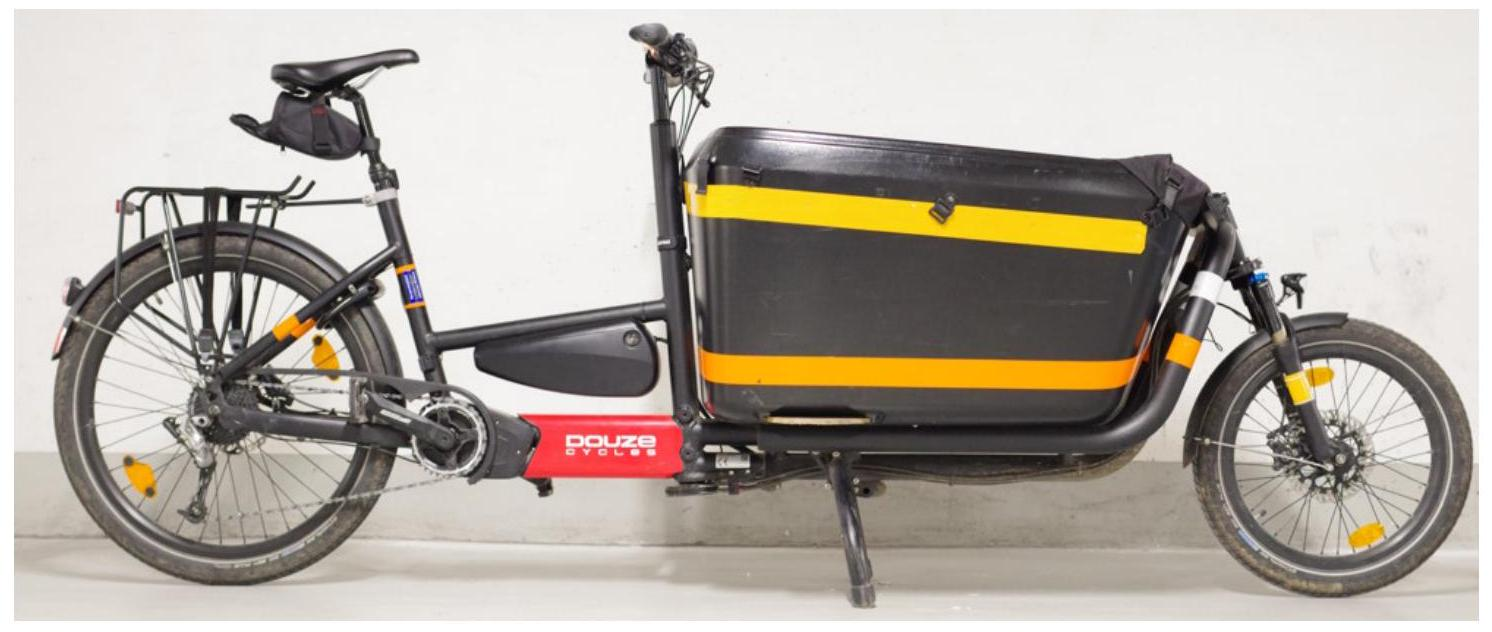
\includegraphics[width=0.8\textwidth]{2024_12_06_8b2ce2e701dae8972925g-01}
\end{center}


Le secteur des transports est la première source d'émissions de gaz à effet de serre en France avec \(31 \%\) des émissions du pays. Ces émissions sont, pour plus de moitié, dues aux véhicules individuels motorisés (voitures, motos) qui restent utilisés au quotidien par \(68 \%\) des Français alors que plus de la moitié des trajets effectués fait moins de \(5 \mathrm{~km}\)\footnote{Données extraites de l’article « Bouger autrement au quotidien » publié par l’ADEME  \url{https://librairie.ademe.fr/cadic/
7338/guide-bouger-autrement-au-quotidien.pdf}}.

À l'inverse, non content d'être un très faible émetteur de gaz à effet de serre, le vélo s'avère peu consommateur en ressources et en énergie tout en étant bon pour la santé individuelle et collective. Le vélo constitue également une solution viable pour décongestionner les villes. Son utilisation est encouragée par de nombreux acteurs institutionnels de par la création d'aménagements cyclables, les aides à l'achat de vélo à assistance électrique ou encore la création du forfait mobilité durable.

L'essor des vélos à assistance électrique (VAE) a libéré de nombreux cyclistes de l'appréhension du relief. Le développement des VAE s'est accompagné de celui des vélos cargos qui permettent d'effectuer des livraisons ou encore de transporter des enfants. Ce sujet porte sur un de ces vélos cargo.

\subsection{Présentation du système}

La société Douze cycles conçoit et réalise des vélos cargo destinés aux professionnels comme aux particuliers. Cette société est implantée en Bourgogne où elle emploie 25 collaborateurs.

Le système étudié est un biporteur à assistance électrique, le G4e, conçu et réalisé par Douze cycles. Soucieuse d'allier durabilité, praticité et esthétique, la société Douze cycles innove continument pour faire évoluer sa gamme de produits. Ce vélo, présenté par l'entreprise comme «une solution vélogistique tout-en-un répondant à la plupart des usages pour les familles ou les professionnels », a été lancé en 2017 pour le cinquième anniversaire de la marque.

\subsection{Étude proposée}
Les études proposées dans ce sujet portent sur différentes problématiques spécifiques à la conception du vélo cargo étudié.

\begin{itemize}
  \item L'étude s'ouvre, partie \ref{ATS_2024_sec2} sur la détermination de l'effort que doit fournir le cycliste pour garer le vélo sur sa béquille.
  \item La partie \ref{ATS_2024_sec3} aborde le dimensionnement des organes de freinage.
  \item La modélisation du capteur utilisé pour mesurer le couple appliqué par le cycliste sur le pédalier occupe la partie \ref{ATS_2024_sec4}.
  \item La partie \ref{ATS_2024_sec5} se focalise sur l'étude de l'association \{ onduleur + machine \} qui anime le groupe d'assistance.
  \item Enfin, les modèles obtenus lors des deux parties précédentes sont exploités partie \ref{ATS_2024_sec6} lors de l'étude de l'asservissement du couple délivré par la machine du groupe d'assistance.\\
Les différentes parties de cette étude sont indépendantes.
\end{itemize}

%\footnotetext{\begin{enumerate}
%  \item Données extraites de l'article « Bouger autrement au quotidien » publié par l'ADEME \href{https://librairie.ademe.fr/cadic/}{https://librairie.ademe.fr/cadic/} 7338/guide-bouger-autrement-au-quotidien.pdf
%\end{enumerate}
%}

\section{Effort de mise en stationnement \label{ATS_2024_sec2}}

\begin{obj}
Déterminer l'effort à exercer par l'usager lors de la mise en stationnement sur béquille.
\end{obj}

La mise en position parking du vélo cargo (le « béquillage») nécessite d'exercer un effort sur le guidon. Cette partie vise à déterminer cet effort et à vérifier sa compatibilité avec les exigences d'ergonomie.\\

\begin{figure}[!htb]
\begin{center}
%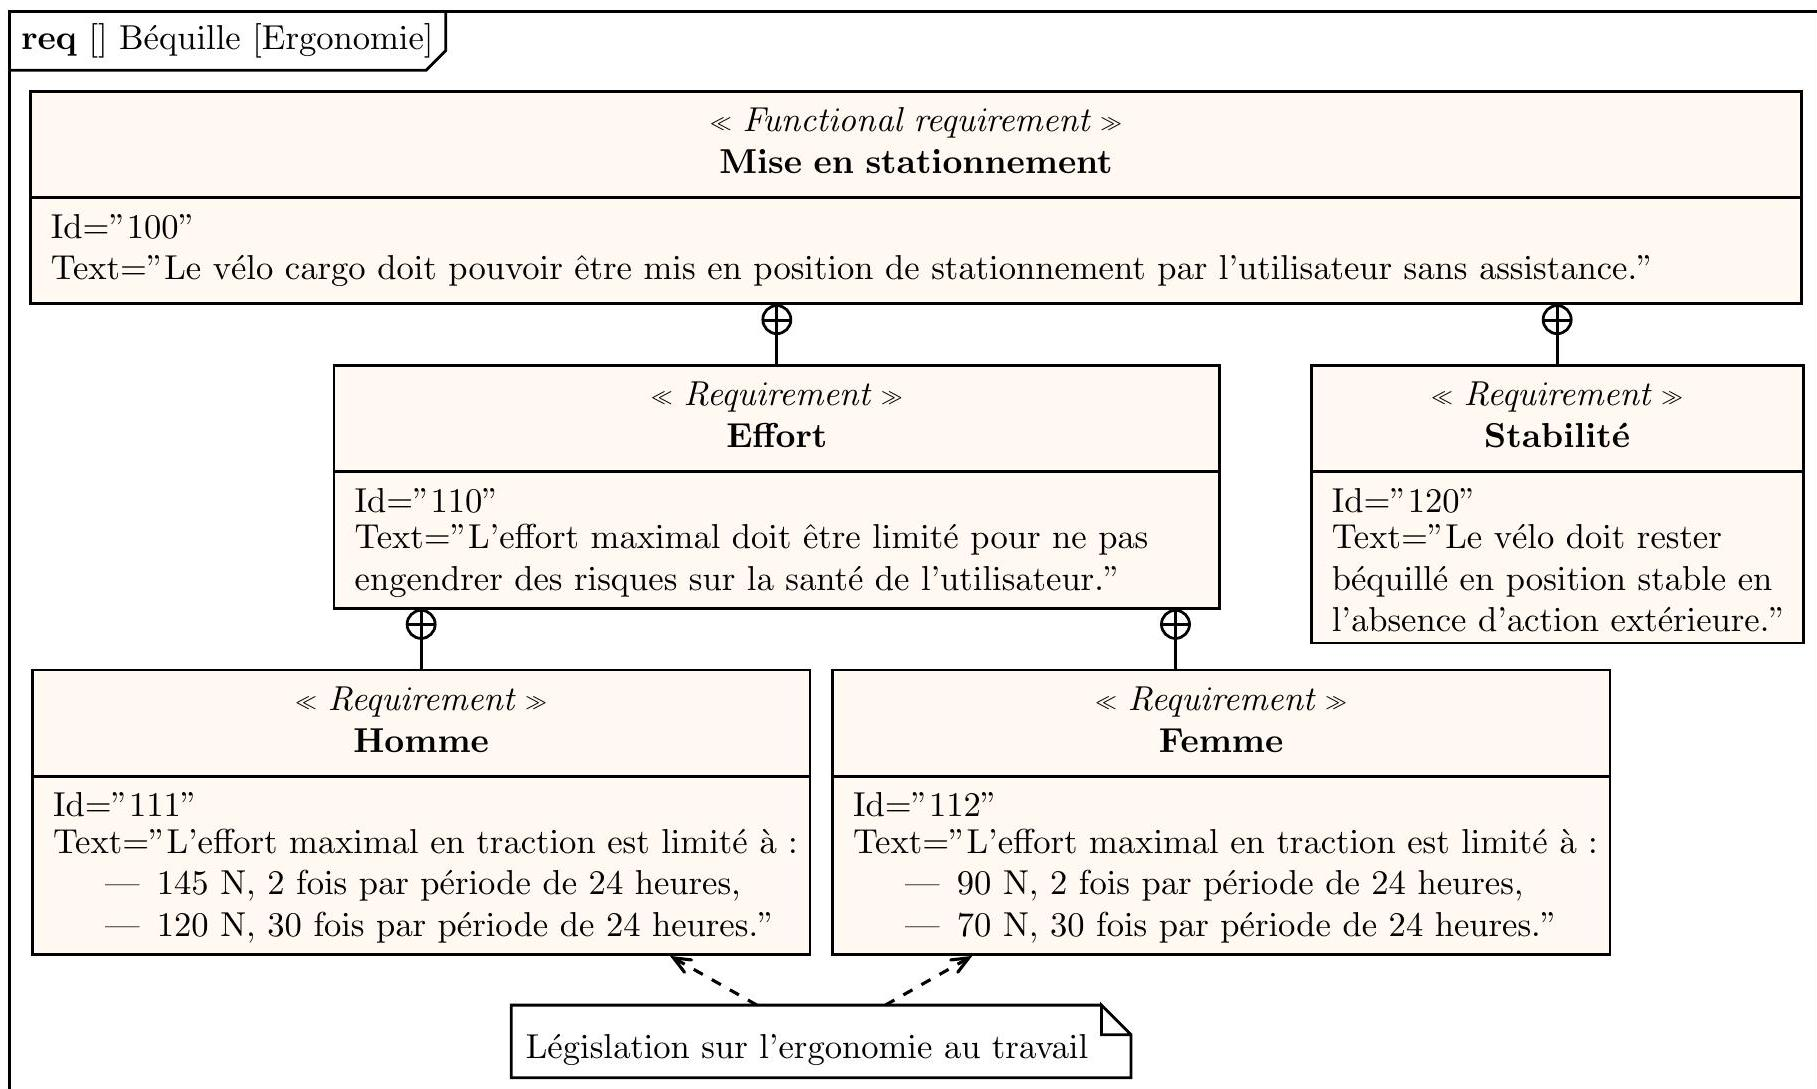
\includegraphics[width=.8\linewidth]{2024_12_06_8b2ce2e701dae8972925g-02}
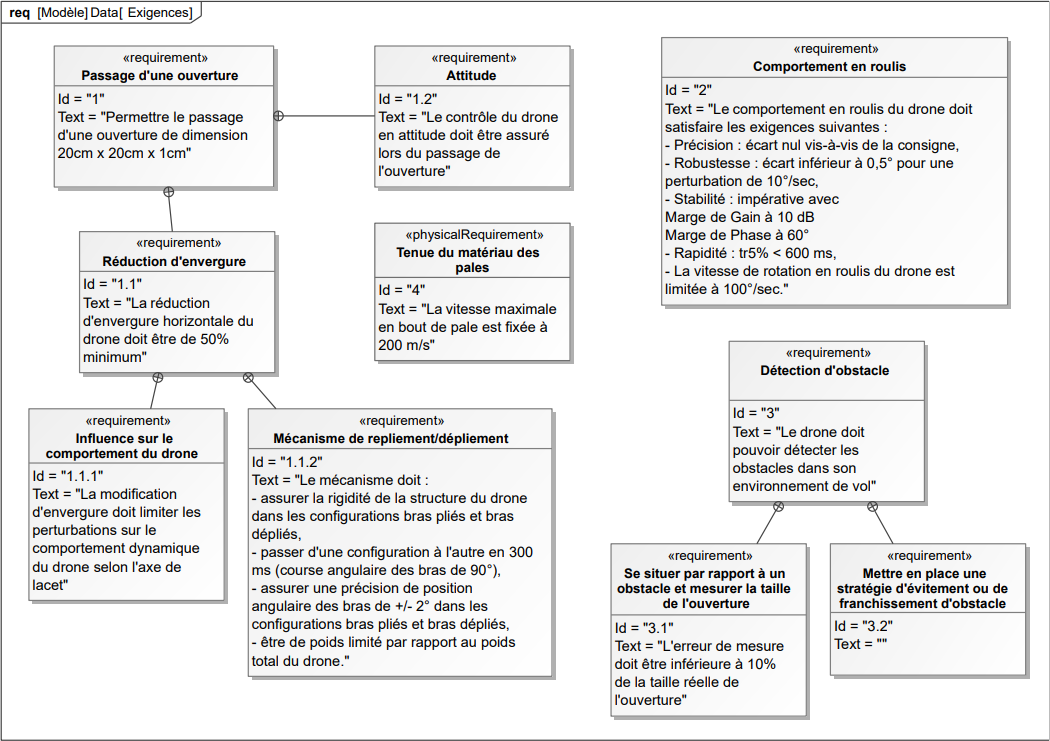
\includegraphics[width=.9\linewidth]{fig_21}
\caption{Extrait du cahier des charges relatif à l'ergonomie de la mise en stationnement du vélo\\ \label{fig2.1}}
\end{center}
\end{figure}

\begin{figure}[!htb]
\begin{center}
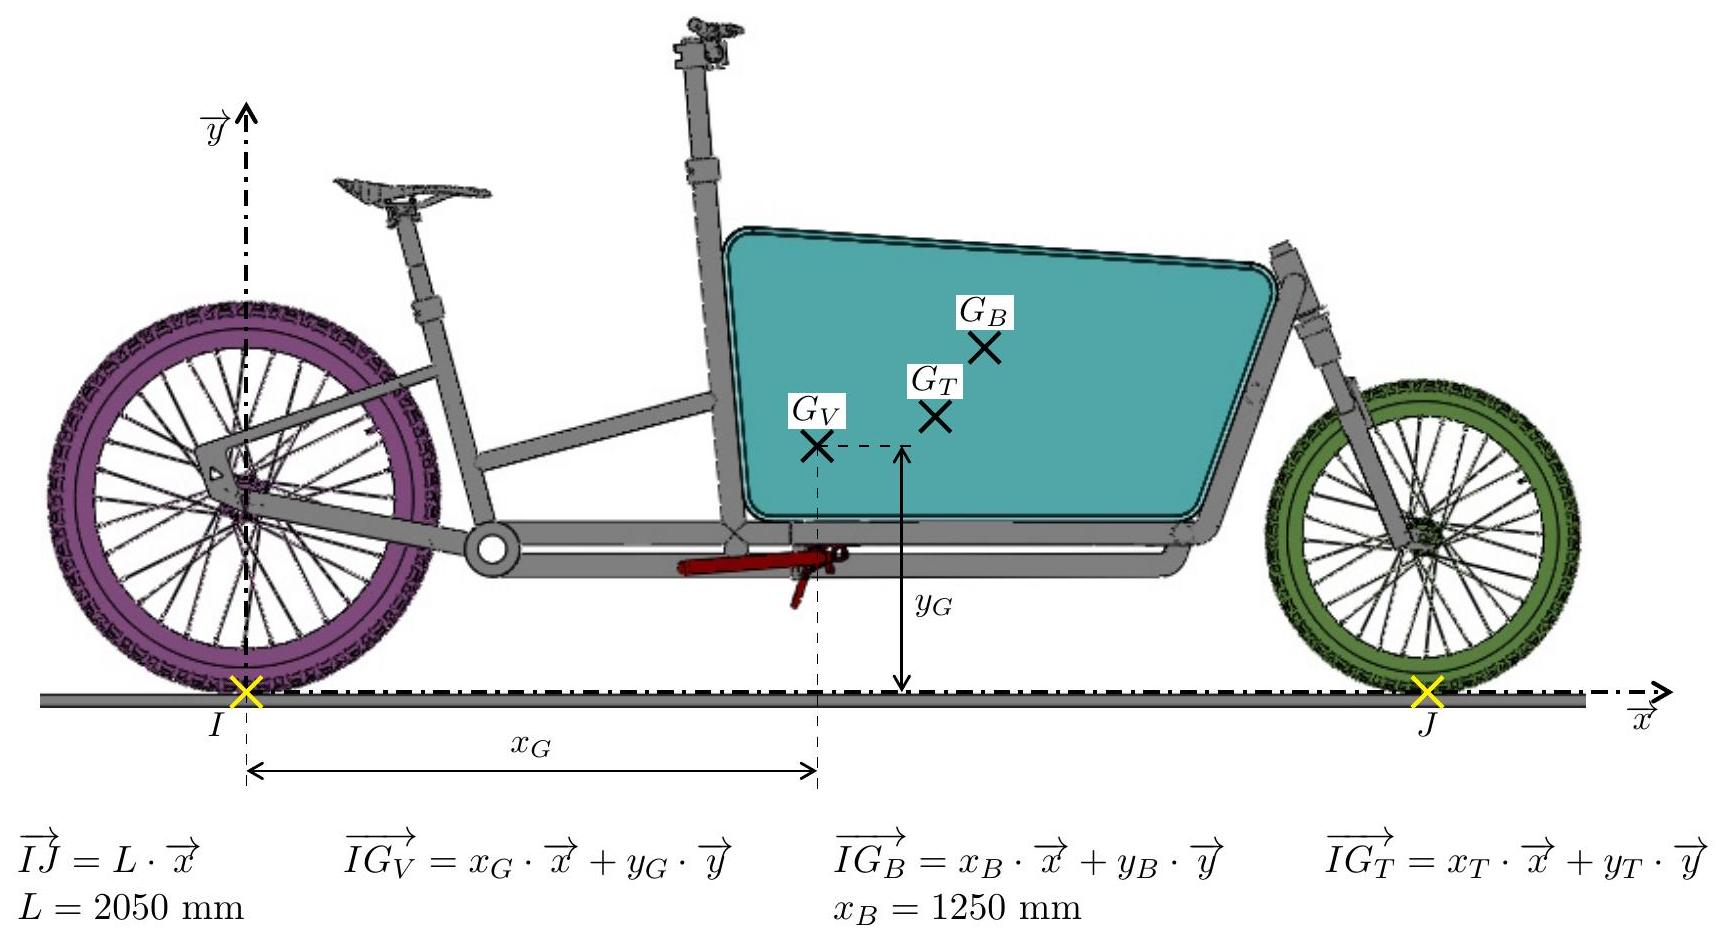
\includegraphics[width=0.8\textwidth]{2024_12_06_8b2ce2e701dae8972925g-02(1)}
\caption{Paramétrage adopté pour la détermination des caractéristiques inertielles du vélo \label{fig2.2}}
\end{center}
\end{figure}


\subsection{Caractéristiques inertielles du vélo}
\paragraph*{Définition des ensembles}
\begin{itemize}
  \item \(V\) : ensemble du vélo hors béquille (supposée de masse négligeable) et hors black-box;
  \item \(B\) : black-box chargée au maximum;
  \item \(T=V \cup B\).
\end{itemize}

\subsubsection{Centre de gravité \(G_{V}\) du vélo à vide}
On étudie le vélo G4e à vide (ensemble \(V\) ). La masse totale de cet ensemble est alors \(m_{V}=49 \mathrm{~kg}\). Les roues du vélo ainsi équipé sont positionnées sur des balances, l'ensemble étant en équilibre dans le plan vertical \((I ; \vec{x}, \vec{y})\). On mesure au niveau des points de contact:
\begin{itemize}
\item arrière, \(I: m_{I}=26 \mathrm{~kg}\);
  \item avant, \(J: m_{J}=23 \mathrm{~kg}\).
\end{itemize}
La distance entre les points \(I\) et \(J\) est notée \(L=2050 \mathrm{~mm}\) (voir figure \ref{fig2.2}).\\


\question{Déterminer l'expression littérale de la position \(x_{G}\) suivant \(\vec{x}\) du centre de gravité de l'ensemble. En déduire la valeur de \(x_{G}\) en mm (on arrondira le résultat à la dizaine de mm ).}

\subsubsection{Centre de gravité \(G_{T}\) du vélo chargé}
On considère à présent que la black box est chargée à son maximum ( \(m_{B}=100 \mathrm{~kg}\) ). On appelle \(G_{B}\), le centre de gravité de la masse chargée où \(x_{B}=1250 \mathrm{~mm}\)

\question{Déterminer l'expression littérale de la position \(x_{T}\) suivant \(\vec{x}\) du centre de gravité de l'ensemble chargé. Calculer la valeur, arrondie à la dizaine de mm , de \(x_{T}\).}

\subsection{Étude géométrique}
L'étude est menée dans le plan \((I ; \vec{x}, \vec{y})\) à partir du paramétrage défini figure \ref{fig_23}.

\paragraph*{Procédure de béquillage} Le béquillage se réalise en poussant la béquille avec le pied sur le sol puis en exerçant une action de traction sur le guidon.

L'utilisateur garde son pied sur la béquille pour la plaquer au sol durant toute la phase de béquillage afin de maintenir le contact en \(K\) de la béquille avec le sol.

\paragraph*{Mouvement du vélo} On suppose dans cette partie que la fourche avant est rigide durant la phase de béquillage. Dès lors, la roue avant se décollera du sol sous l'action de traction du vélo par l'usager tandis que la roue arrière reculera.

\paragraph*{Définition de l'ensemble étudié :} L'ensemble étudié se compose des solides suivants :
\begin{itemize}
  \item le sol (0), repère associé ( \(I ; \vec{x}, \vec{y}, \vec{z})\);
  \item la roue arrière (1);
  \item le cadre (2), repère associé \(\left(A ; \overrightarrow{x_{c}}, \overrightarrow{y_{c}}, \vec{z}\right)\);
  \item la béquille (4), repère associé \(\left(A ; \overrightarrow{x_{b}}, \overrightarrow{y_{b}}, \vec{z}\right)\);
  \item la roue avant (3).
\end{itemize}

\paragraph*{Modèle cinématique} On modélise la cinématique de l'ensemble par une liaison :

\begin{itemize}
  \item sphère/plan en \(I\) suivant \(\vec{y}\) entre la roue arrière (1) et le sol (0);
  \item pivot d'axe ( \(B ; \vec{z}\) ) entre la roue (1) et le cadre (2);
  \item pivot d'axe \((A ; \vec{z})\) entre le cadre (2) et la béquille (4);
  \item pivot d'axe \((K ; \vec{z})\) entre la béquille (4) et le sol (0) (modélisation associée au blocage de la béquille par le pied);\\
\end{itemize}

\begin{figure}[!htb]
\centering

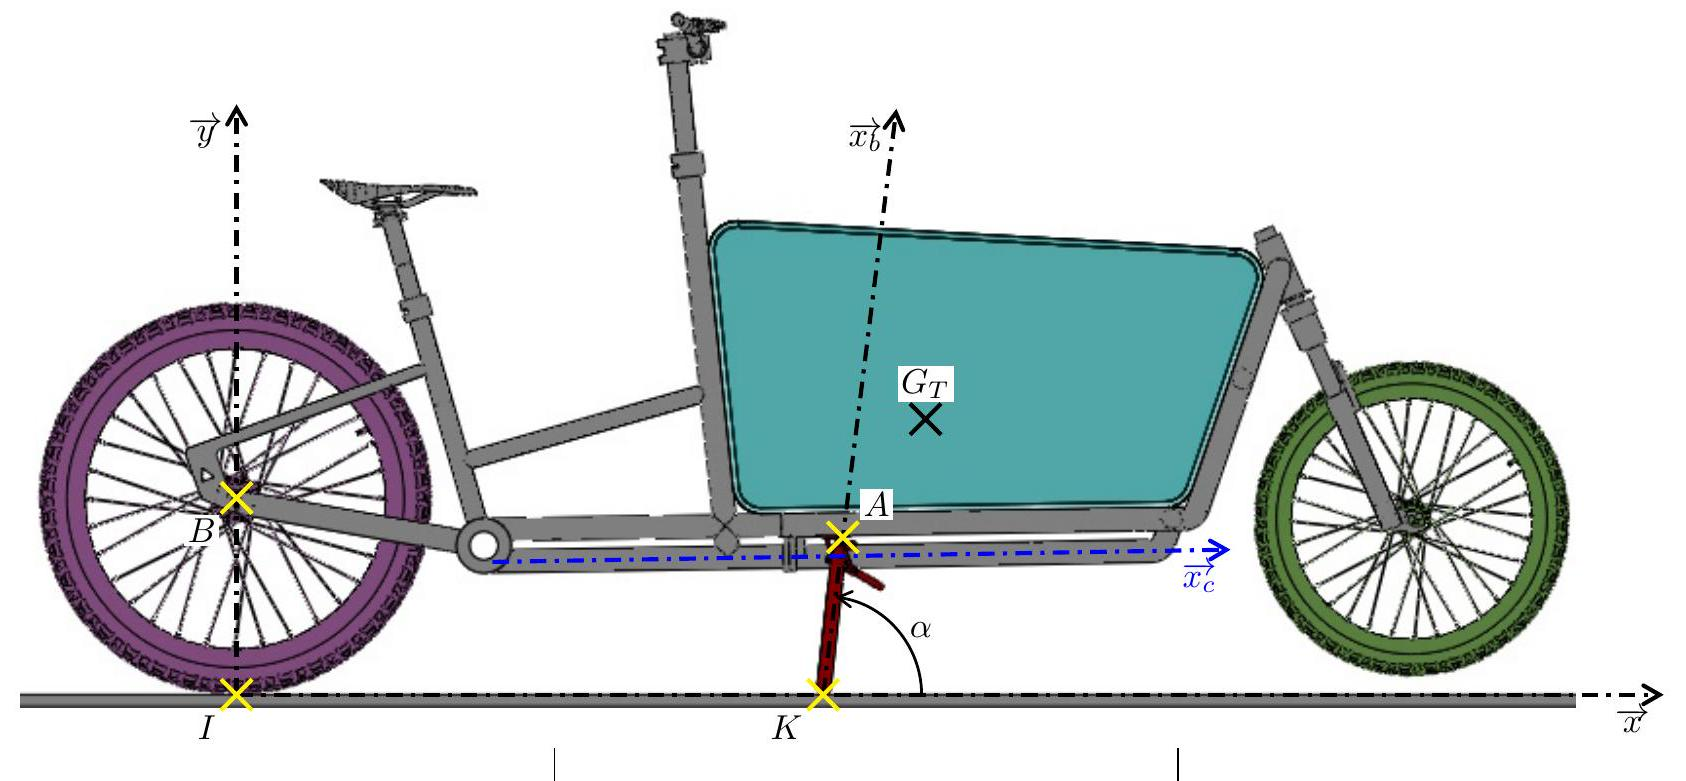
\includegraphics[width=0.8\textwidth]{2024_12_06_8b2ce2e701dae8972925g-04(1)}

\begin{tabular}{p{5cm}p{5cm}p{5cm}}
$
\begin{aligned}
\overrightarrow{K I} & =\mu(t) \cdot \vec{x} \\
\overrightarrow{K A} & =a \cdot \overrightarrow{x_{b}} \\
\overrightarrow{I B} & =R_{B} \cdot \vec{y} \\
\overrightarrow{A B} & =-b \cdot \overrightarrow{x_{c}}+e \cdot \overrightarrow{y_{c}} \\
\overrightarrow{A G_{T}} & =\left(x_{T}-b\right) \cdot \overrightarrow{x_{c}}+\left(y_{T}-h\right) \cdot \overrightarrow{y_{c}}
\end{aligned}
$
&
$
\begin{aligned}
a & =290 \mathrm{~mm} \\
R_{B} & =340 \mathrm{~mm} \\
b & =1030 \mathrm{~mm} \\
e & =70 \mathrm{~mm} \\
h & =270 \mathrm{~mm} \\
x_{T} & =1150 \mathrm{~mm} \\
y_{T} & =400 \mathrm{~mm}
\end{aligned}
$
&
$
\begin{aligned}
& \alpha(t)=\left(\vec{x}, \overrightarrow{x_{b}}\right)=\left(\vec{y}, \overrightarrow{y_{b}}\right) \\
& \beta(t)=\left(\vec{x}, \overrightarrow{x_{c}}\right)=\left(\vec{y}, \overrightarrow{y_{c}}\right)
\end{aligned}
$
La partie basse du cadre est à l'horizontale avant le béquillage : \(\overrightarrow{x_{c}}\) et \(\vec{x}\) sont colinéaires lorsque les deux roues sont en contact avec le sol.
\\
\end{tabular}
% FIG 2.3
\caption{\label{fig_23} Paramétrage utilisé pour l'étude du béquillage}

\end{figure}



\question{Compléter le schéma cinématique esquissé sur le document réponse A conformément au modèle proposé en faisant apparaître les liaisons, les solides et les repères qui leurs sont associés.}

\question{Compléter les figures de calcul esquissées sur le document réponse B.}

\question{À partir d'une fermeture géométrique, montrer que l'équation scalaire qui lie la valeur de \(\beta\) à \(\alpha, a, b, e\) et \(R_{B}\) est de la forme : \(a \cdot \sin (\alpha)=b \cdot \sin (\beta)-e \cdot \cos (\beta)+R_{B}\).}

\paragraph*{Valeurs limites de \(\alpha\)} On note \(\alpha_{i}\) et \(\alpha_{f}\left(\alpha_{i}<\alpha_{f}\right)\) les valeurs de l'angle \(\alpha\) entre lesquelles la roue avant est décollée du sol.

\question{Déterminer les expressions des angles \(\alpha_{i}\) et \(\alpha_{f}\) en fonction de \(R_{B}\), e et \(a\). En calculer les valeurs en radians.}

Les valeurs calculées précédemment arrondies conduisent à \(\alpha_{i} \approx 70^{\circ}\) et \(\alpha_{f} \approx 110^{\circ}\). L'évolution de l'angle \(\beta\) en fonction de \(\alpha\), pour la plage de béquillage, est donnée figure \ref{fig_24}.

\question{Déduire de la courbe fournie la valeur d'inclinaison maximale du cadre par rapport au sol, notée \(\beta_{\max }\). Conclure sur l'hypothèse d'étude suivante : «Le cadre sera supposé horizontal lors du béquillage ».}

\begin{figure}[!htb]
\begin{center}
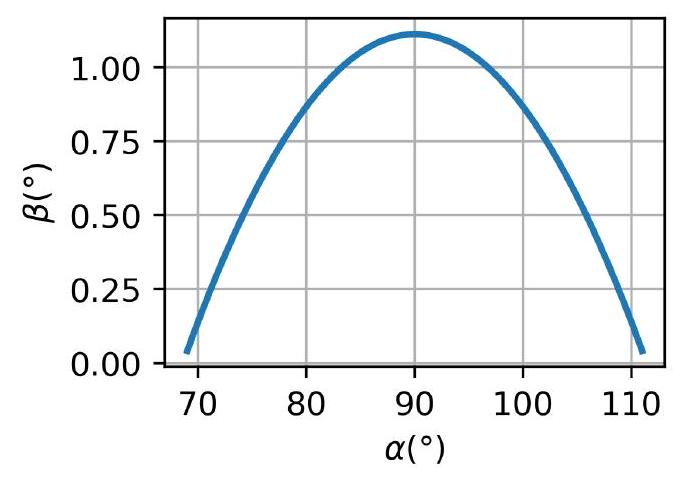
\includegraphics[width=.4\linewidth]{2024_12_06_8b2ce2e701dae8972925g-04}
\caption{Évolution de \(\beta\) en fonction de \(\alpha\) au cours du béquillage. \label{fig_24}}
\end{center}
\end{figure}


\subsection{Effort de béquillage}
On se propose à présent d'estimer l'action mécanique que doit développer le cycliste sur le guidon lors du béquillage dans le cas où la béquille est perpendiculaire au cadre ( \(\alpha=90^{\circ}\), on admet qu'il s'agit de la position critique en termes d'effort). Le paramétrage adopté pour cette étude est défini figure \ref{fig_25}.\\

\begin{figure}[!htb]
\begin{center}
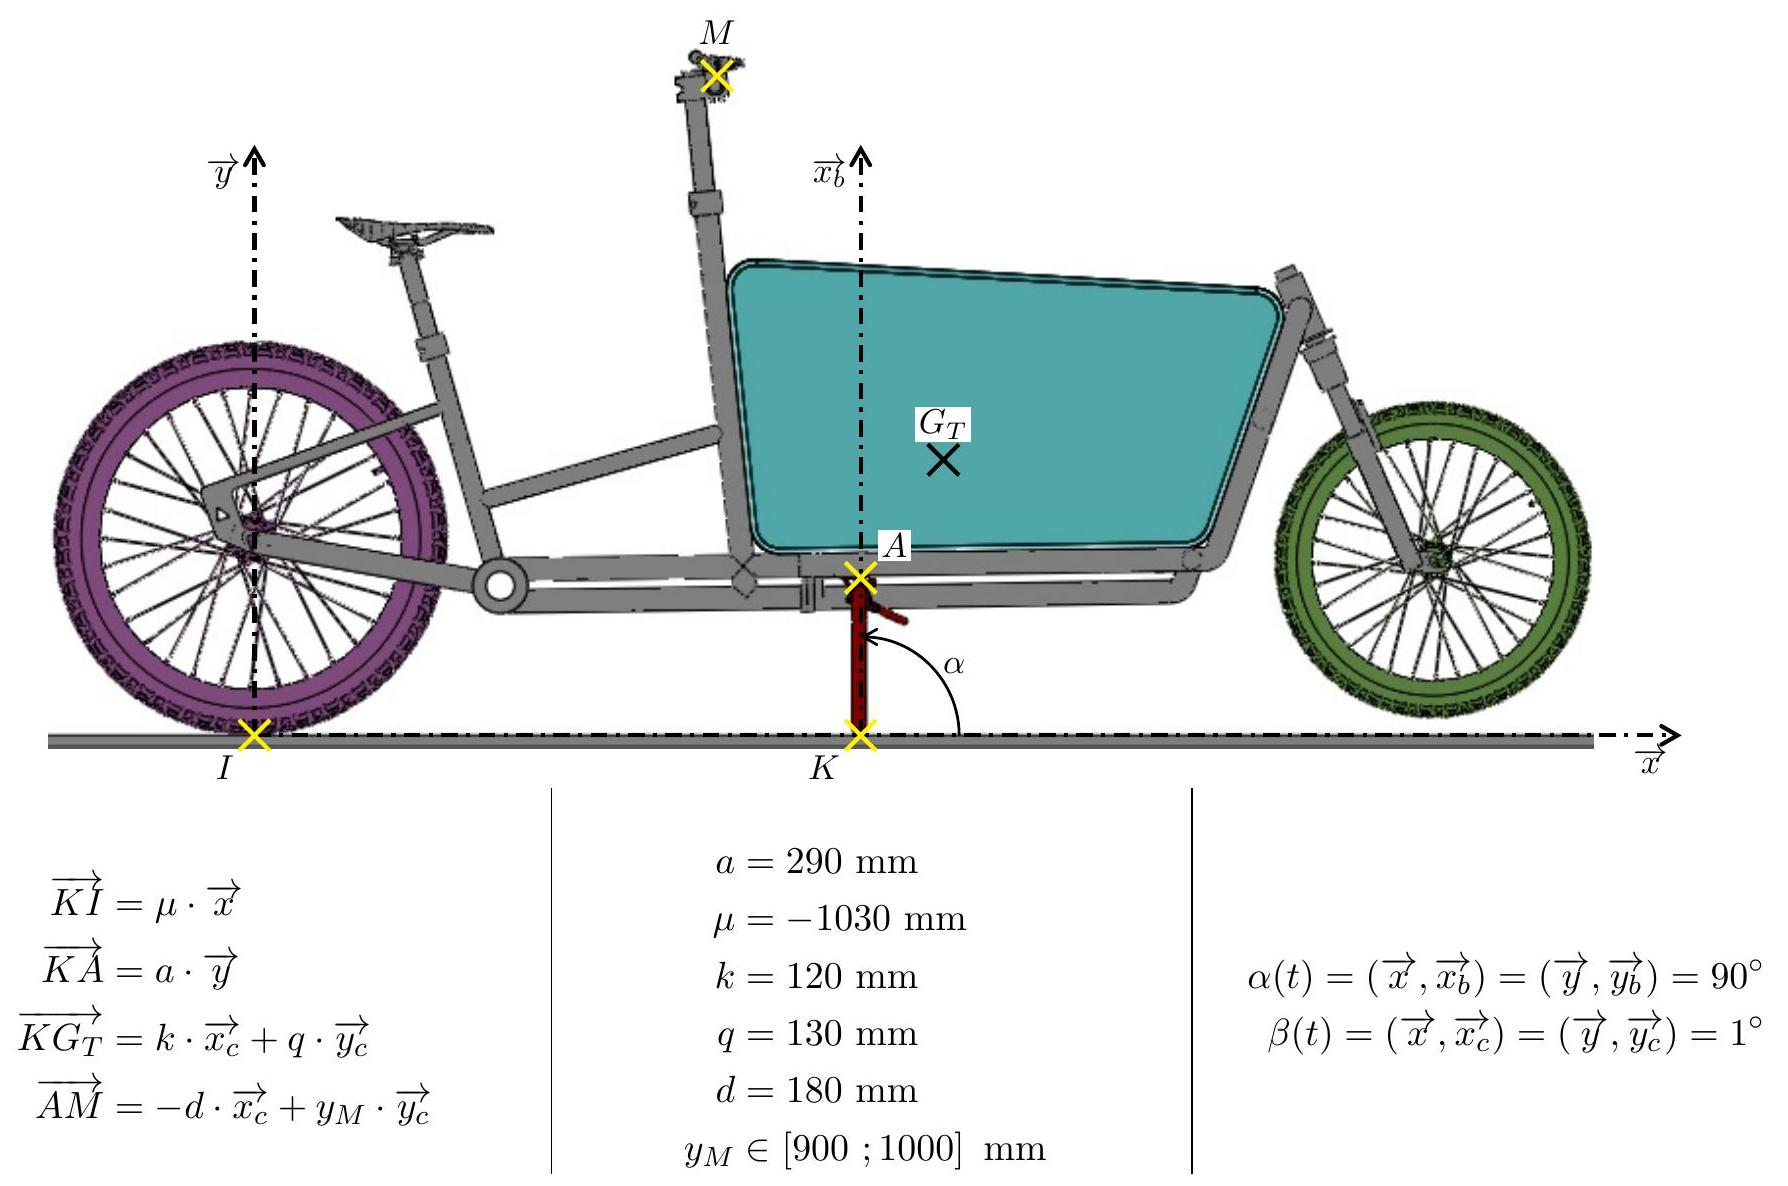
\includegraphics[width=0.8\textwidth]{2024_12_06_8b2ce2e701dae8972925g-05}
\caption{Paramétrage utilisé pour la détermination de l'effort à appliquer sur le guidon \label{fig_25}}
\end{center}
\end{figure}


Notation Le torseur de l'action mécanique exercée par le solide \(i\) sur \(j\), dans la base ( \(\vec{x}, \vec{y}, \vec{z}\) ), dans l'hypothèse de problème plan, est noté :
$
\{i \rightarrow j\}=\left\{\begin{array}{c|c}
X_{i j} & - \\
Y_{i j} & - \\
- & N_{i j}^{K}
\end{array}\right\}_{(\vec{x}, \vec{y}, \vec{z})} \quad \text { ou } \quad\{i \rightarrow j\}=_{K}\left\{\begin{array}{c}
X_{i j} \cdot \vec{x}+Y_{i j} \cdot \vec{y} \\
N_{i j}^{K} \cdot \vec{z}
\end{array}\right\}
$

\paragraph*{Données et hypothèses}
\begin{itemize}
  \item L'action mécanique exercée par le cycliste est un glisseur \(\overrightarrow{F_{C}}\) appliqué en \(M\) tel que \(\overrightarrow{F_{C}}=-F_{C} \cdot \vec{x}\).
  \item L'accélération de la pesanteur vaut \(\vec{g}=-g \cdot \vec{y}\) où on approche \(g\) par \(g=10 \mathrm{~m} / \mathrm{s}^{2}\).
  \item La masse de l'ensemble, pour rappel, est notée \(m_{T}\) et vaut \(m_{T}=149 \mathrm{~kg}\).
  \item On suppose les liaisons sans frottements à l'exception du contact Roue/Sol, où l'on suppose un frottement suivant le modèle de Coulomb de coefficient \(f=1\).
\end{itemize}

\question{Donner la forme du torseur des actions mécaniques transmissibles du sol ( 0 ) sur la béquille (4) en \(K\) dans la base ( \(\vec{x}, \vec{y}, \vec{z})\).}

\question{Donner la forme du torseur des actions mécaniques transmissibles du sol (0) sur la roue (1) en \(I\) dans la base \((\vec{x}, \vec{y}, \vec{z})\).}

\question{Donner la forme du torseur des actions mécaniques exercées par la pesanteur sur l'ensemble \(\Sigma=\{1,2,3,4\}\) en \(G_{T}\) dans la base ( \(\vec{x}, \vec{y}, \vec{z}\) ).}

\question{Appliquer le théorème du moment statique à \(\Sigma\) en \(I\) en projection sur \(\vec{z}\). En déduire la relation qui lie \(F_{C}\) à \(Y_{04}\) en fonction de \(\mu, a, k, q, d, y_{M}, \beta, m_{T}\) et \(g\).}

On suppose que \(\beta\) est suffisamment petit pour considérer que \(\sin \beta \approx 0\) et \(\cos \beta \approx 1\).\\



\question{Montrer qu'alors, on peut exprimer \(F_{C}\) sous la forme :
$
F_{C} \approx \dfrac{\mu \cdot Y_{04}-(\mu-k) \cdot m_{T} \cdot g}{y_{M}+a}
$.
Déterminer la condition sur \(y_{M}\) qui conduit alors à une action à développer par le cycliste \(F_{C}\) maximale.}

\question{En isolant l'ensemble \(\Sigma\) et en appliquant le théorème de la résultante statique, écrire les équations scalaires qui relient les différentes composantes des torseurs d'actions mécaniques exercées par le sol.}

\question{Montrer alors, que même en supposant le glissement en \(I\), l'isolement de l'ensemble ne permet pas de déterminer l'action du cycliste.}

On se propose à présent d'isoler la béquille (4) seule. On fait l'hypothèse que son poids est négligeable devant les autres actions mécaniques.

\question{Montrer en appliquant le PFS à la béquille (4) et en choisissant une équation scalaire pertinente parmi celles disponibles, que pour la position étudiée ( \(\alpha=90^{\circ}\) ) et pour l'isolement choisi, \(X_{03}=0\).}

On montre alors en utilisant les résultats précédents :
$
F_{C}=\dfrac{f \cdot k \cdot m_{T} \cdot g}{\mu+f \cdot\left(y_{M}+a\right)}
$.

On estime alors l'effort minimal pour assurer le béquillage en charge maximale à \(F_{C} \approx 80 \mathrm{~N}\).

\question{Conclure sur le respect de l'exigence 110 du cahier des charges du vélo (figure \ref{fig2.1}).}

\section{Vérification du dimensionnement des organes participant au freinage}
La sécurité des utilisateurs du vélo cargo passe par un freinage performant. Les pneumatiques et les freins doivent garantir une distance d'arrêt du vélo raisonnable même lorsque celui-ci est chargé au maximum. L'étude proposée dans cette partie vise à vérifier le dimensionnement de ces éléments à la lumière du cahier des charges précisé dans le diagramme des exigences de la figure \ref{fig_3_cargo}.

\begin{figure}[!h]
\centering
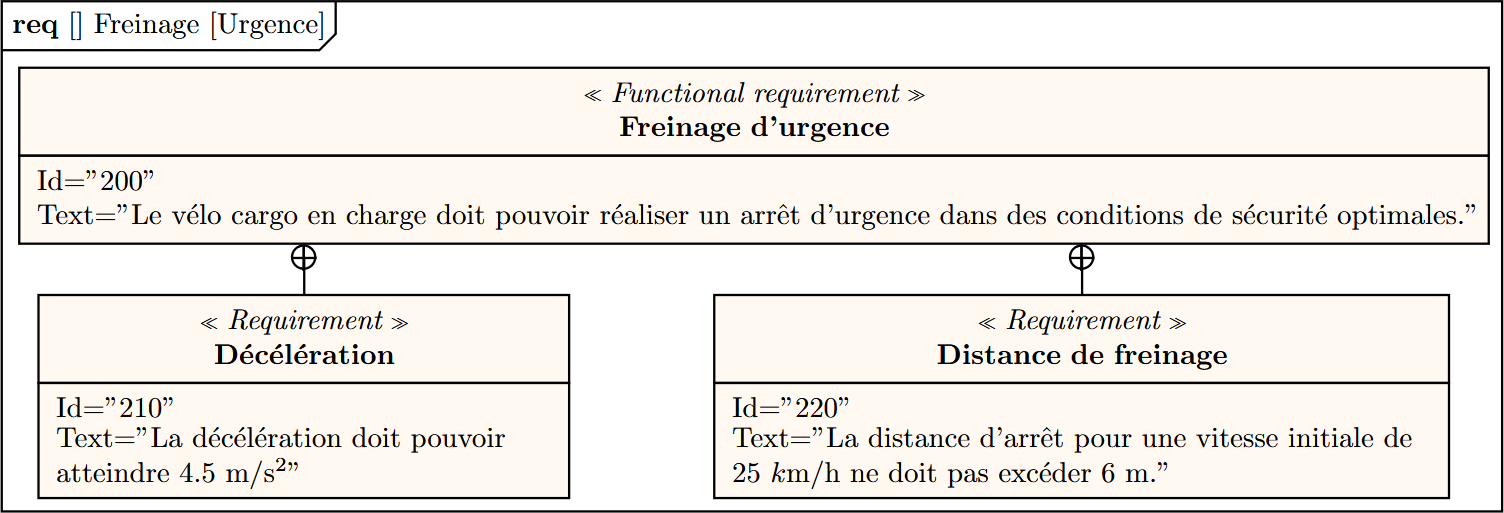
\includegraphics[width=.8\linewidth]{fig_31}
\caption{\label{fig_3_cargo}Extrait du cahier des charges relatif au freinage d'urgence}
\end{figure}





\subsection{Modèle d'étude}
\subsubsection{Définition des ensembles}
On étudie le vélo G4 muni de sa «black box», chargé à son maximum et en mouvement de translation rectiligne dans la direction \(\vec{x}\) (figure \ref{fig_32}). Le cadre est supposé horizontal et la fourche avant est infiniment rigide. Les différents ensembles définis pour l'étude du freinage sont listés dans le tableau \ref{tab_31}. Ces ensembles sont supposés indéformables. Leurs caractéristiques inertielles sont recensées dans le tableau \ref{tab_32}.

Le repère associé au sol (0) est supposé galiléen.

\subsubsection{Modélisation des contacts entre les ensembles}
\paragraph*{Contact roues-sol} 
Les contacts entre les roues et le sol sont modélisés par des liaisons sphère-plan. Le frottement est pris en compte au niveau de ces contacts, la résistance au roulement est négligée, ainsi :

$
\begin{aligned}
& \{0 \rightarrow 1\}=_{I}\left\{\begin{array}{c}
-X_{01} \cdot \vec{x}+Y_{01} \cdot \vec{y} \\
\overrightarrow{0}
\end{array}\right\} \quad \text { où }\left\{\begin{array} { c } 
{ X _ { 0 1 } > 0 } \\
{ Y _ { 0 1 } > 0 }
\end{array} \quad \text { et } \left\{\begin{array}{rl}
\text { si glissement en } I: & X_{01}=f^{\prime} \cdot Y_{01} \\
\text { si non glissement en } I: & X_{01}<f^{\prime} \cdot Y_{01}
\end{array}\right.\right. \\
& \{0 \rightarrow 3\}={ }_{J}\left\{\begin{array}{c}
-X_{03} \cdot \vec{x}+Y_{03} \cdot \vec{y} \\
\overrightarrow{0}
\end{array}\right\} \quad \text { où }\left\{\begin{array} { c } 
{ X _ { 0 3 } > 0 } \\
{ Y _ { 0 3 } > 0 }
\end{array} \quad \text { et } \left\{\begin{array}{rl}
\text { si glissement en } J: & X_{03}=f^{\prime} \cdot Y_{03} \\
\text { si non glissement en } J: & X_{03}<f^{\prime} \cdot Y_{03}
\end{array}\right.\right.
\end{aligned}
$

où \(f^{\prime}\) désigne, selon la configuration, le coefficient de frottement ou d'adhérence du contact roue-sol (supposés égaux). La valeur de \(f^{\prime}\) dépend de nombreux facteurs parmi lesquels l'état du pneumatique et l'humidité de la chaussée (voir tableau \ref{tab_33}).

\paragraph*{Guidages en rotation des roues} Les roues sont en liaison pivot avec l'ensemble (2) :

\begin{itemize}
  \item autour de l'axe \((B, \vec{z})\) pour la roue arrière (1),
  \item autour de l'axe \((C, \vec{z})\) pour la roue avant (3).
\end{itemize}

Ces liaisons sont supposées parfaites.

\paragraph*{Action des freins} Lors du freinage commandé par le cycliste, les freins appliquent sur chaque roue un couple de freinage défini par :
\begin{itemize}
\item pour la roue arrière : \(\overrightarrow{C_{f, 2 \rightarrow 1}}=C_{f 1} \cdot \vec{z}\);
\item pour la roue avant : \(\overrightarrow{C_{f, 2 \rightarrow 3}}=C_{f 3} \cdot \vec{z}\).
\end{itemize}


\begin{table}[!h]
\centering
\begin{tabular}{lll}
Identifiant & Définition & Repère associé \\
\hline
\((0)\) & Sol & \((O ; \vec{x} ; \vec{y} ; \vec{z})\) \\
\((1)\) & Roue arrière & \(\left(B ; \overrightarrow{x_{1}} ; \overrightarrow{y_{1}} ; \vec{z}\right)\) \\
\((2)\) & Vélo privé de ses roues + pilote + charge & \(\left(G_{2} ; \vec{x} ; \vec{y} ; \vec{z}\right)\) \\
\((3)\) & Roue avant & \(\left(C ; \overrightarrow{x_{3}} ; \overrightarrow{y_{3}} ; \vec{z}\right)\) \\
\hline
\end{tabular}
%Tableau 3.1 - 
\caption{Ensembles définis pour l'étude du freinage \label{tab_31}}
\end{table}




\begin{figure}[!htb]
\begin{center}
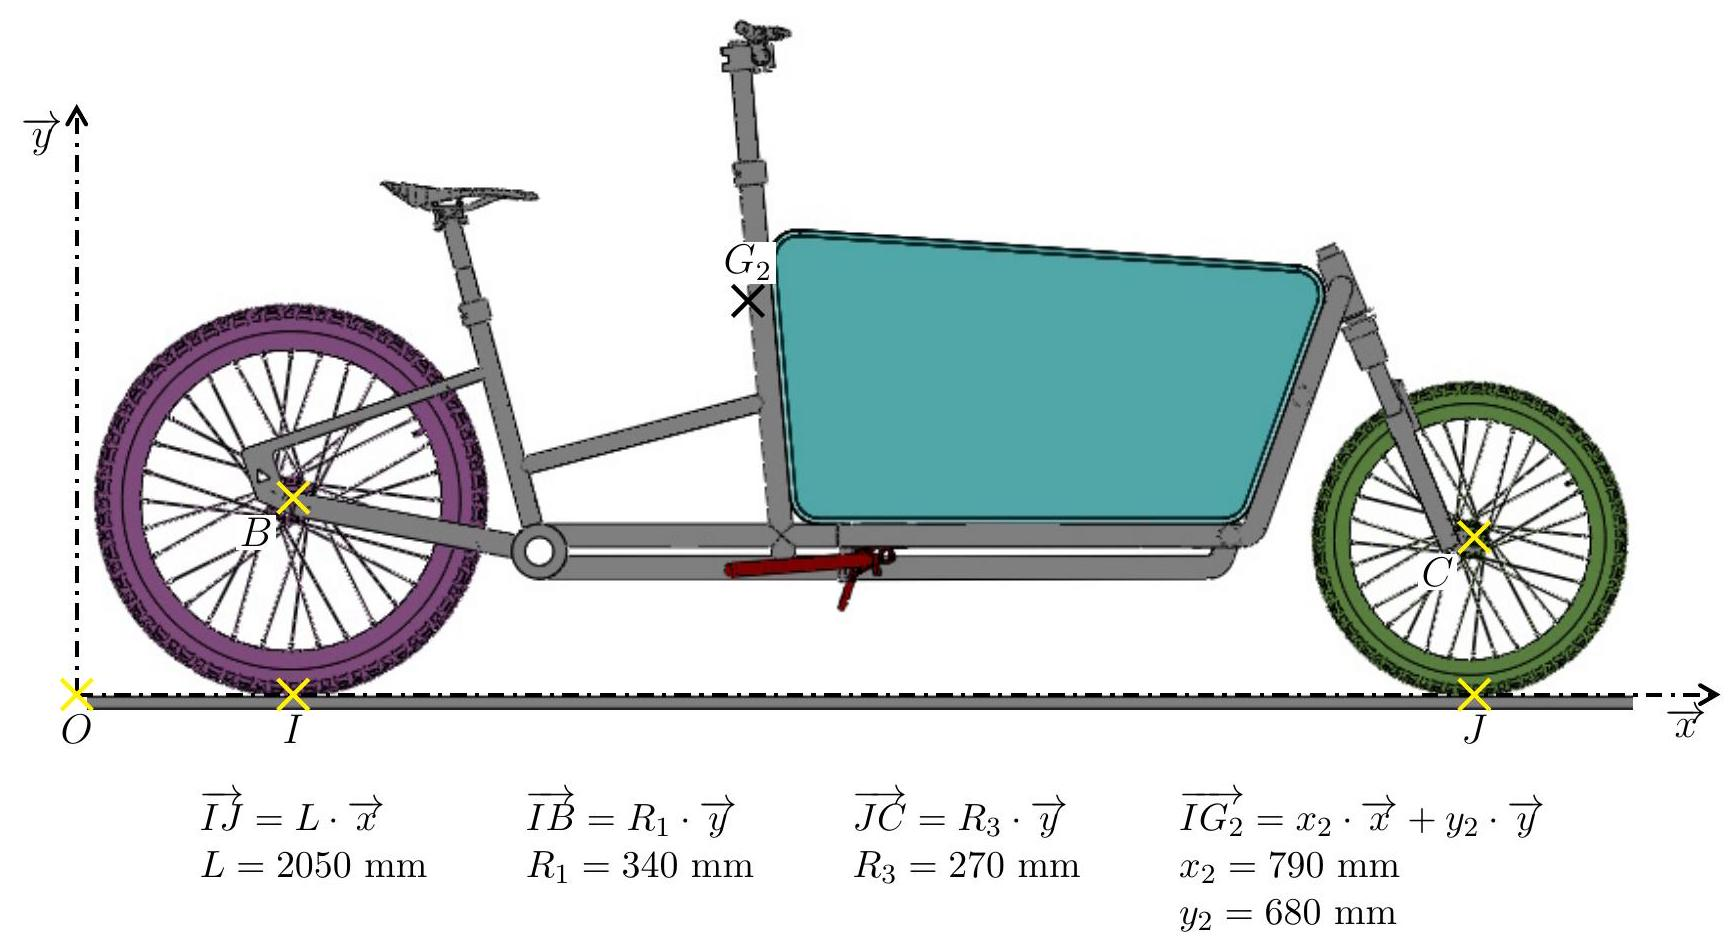
\includegraphics[width=0.8\textwidth]{2024_12_06_8b2ce2e701dae8972925g-08}
% FIG 3.2
\caption{Paramétrage adopté pour le dimensionnement des organes de freinage \label{fig_32}}
\end{center}
\end{figure}


\begin{table}[!h]
\centering
\begin{tabular}{cccc}
Ensemble & Masse & \begin{tabular}{c}
Centre \\
d'inertie \\
\end{tabular} & \begin{tabular}{c}
Moment d'inertie au centre \\
d'inertie suivant \((\vec{z})\) \\
\end{tabular} \\
\hline
Roue arrière (1) & \(m_{1}=8 \mathrm{~kg}\) & \(B\) & \(I_{B 1}=0.78 \mathrm{~kg} \cdot \mathrm{~m}^{2}\) \\
\hline
\begin{tabular}{c}
Ensemble \(\{\) Vélo privé de ses \\
roues + pilote + charge \(\}(2)\) \\
\end{tabular} & \(m_{2}=245 \mathrm{~kg}\) & \(G_{2}\) & - \\
\hline
Roue avant (3) & \(m_{3}=4 \mathrm{~kg}\) & \(C\) & \(I_{C 3}=0.26 \mathrm{~kg} \cdot \mathrm{~m}^{2}\) \\
\hline
\end{tabular}
%Tableau 3.2
\caption{ Caractéristiques inertielles des ensembles pour l'étude du freinage \label{tab_32}}
\end{table}


\begin{table}[!h]
\centering
\begin{tabular}{rcc}
 & Pneu neuf & Pneu anormalement usé \\
\hline
Route goudronnée sèche & 0.8 & 0.95 \\
\hline
Route goudronnée mouillée & 0.6 & 0.3 \\
\hline
\end{tabular}
%Tableau 3.3 - 
\caption{Valeurs du coefficient de frottement/d'adhérence (supposés égaux) \(f^{\prime}\) en fonction de l'état du pneu et de la route \label{tab_33}}
\end{table}


\subsubsection{Grandeurs cinématiques}
\paragraph*{Vitesses de pivotement des roues} On note \(\omega_{12}\) et \(\omega_{32}\) les vitesses de rotation telles que :
$
\overrightarrow{\Omega(1 / 2)}=\omega_{12} \cdot \vec{z} \quad \text { et } \quad \overrightarrow{\Omega(3 / 2)}=\omega_{32} \cdot \vec{z}
$

\paragraph*{Position, vitesse et accélération du point \(G_{2}\) par rapport au sol}
\begin{itemize}
\item La position selon \(\vec{x}\) du point \(G_{2}\) dans le repère du sol (0) est notée \(x_{G_{2}}: x_{G_{2}}(t)=\overrightarrow{O G_{2}} \cdot \vec{x}\);
  \item La vitesse horizontale de \(G_{2}\) est notée \(v_{G_{2}}: v_{G_{2}}(t)=\dfrac{\mathrm{d} x_{G_{2}}(t)}{\mathrm{d} t}\);
  \item L'accélération horizontale du point \(G_{2}\) est désignée par \(\gamma_{G_{2}}: \gamma_{G_{2}}(t)=\dfrac{\mathrm{d} v_{G_{2}}(t)}{\mathrm{d} t}\).
\end{itemize}

\subsection{Capacité de freinage d'urgence}
\begin{obj}
Déterminer les conditions portant sur les pneumatiques qui permettent d'assurer un freinage d'urgence conforme aux exigences de la figure \label{fig_31}.
\end{obj}

\question{Déterminer l'expression des résultantes dynamiques :}
\textit{
\begin{enumerate}
  \item du solide (1) dans son mouvement par rapport au sol (0) : \(\overrightarrow{R_{d}(1 / 0)}\),
  \item de l'ensemble (2) dans son mouvement par rapport au sol (0) : \(\overrightarrow{R_{d}(2 / 0)}\),
  \item du solide (3) dans son mouvement par rapport au sol (0) : \(\overrightarrow{R_{d}(3 / 0)}\).
\end{enumerate}}


\question{ En appliquant le théorème de la résultante dynamique au système matériel \(\{1,2,3\}\), déterminer les expressions :}
\textit{
\begin{itemize}
  \item de la somme des composantes tangentielles \(\left(X_{01}+X_{03}\right)\) et
  \item de la somme des composantes normales \(\left(Y_{01}+Y_{03}\right)\)
de l'action du sol sur les roues.
\end{itemize}}

On se propose d'équilibrer la répartition du freinage de telle façon que les composantes tangentielles exercées par le sol sur les roues soient identiquement proportionnelles aux composantes normales. On introduit dès lors le coefficient \(k_{f}\) de proportionnalité correspondant tel que :
$
X_{01}=k_{f} \cdot Y_{01} \quad \text { et } \quad X_{03}=k_{f} \cdot Y_{03}
$

\question{Déterminer une expression de \(k_{f}\) en fonction de \(g\) et \(\gamma_{G_{2}}\).}

\question{À partir de l'expression de la condition de non glissement des roues sur le sol, déterminer la valeur limite de \(\gamma_{G_{2}}(t)\) en fonction de \(f^{\prime}\) et \(g\). Montrer alors que toutes les configurations du tableau 3.3 ne permettent pas de satisfaire l'exigence 210.}

On considère à présent uniquement la situation où le freinage peut être réalisé sans glissement. Quels que soient les résultats trouvés précédemment, on définit deux valeurs pour la décélération limite \(\gamma_{l i m}\) :

\begin{itemize}
  \item \(\gamma_{\text {lim }}=-4.5 \mathrm{~m} \cdot \mathrm{~s}^{-2}\) dans le cas du freinage en conditions normales (pneus neufs ou pneus usés sur chaussée sèche),
  \item \(\gamma_{\text {lim }}=-2.95 \mathrm{~m} \cdot \mathrm{~s}^{-2}\) dans le cas du freinage en conditions dégradées (pneus usés sur chaussée mouillée).
\end{itemize}

On suppose de plus que la décélération maximale est immédiatement atteinte lorsque l'utilisateur agit sur les freins. La décélération est supposée constante pendant toute la durée du freinage.


\question{En étudiant le mouvement de l'ensemble \(\{1,2,3\}\) lors du freinage, montrer que la distance de freinage \(d_{f}\) définie par le passage de la vitesse initiale \(v_{0}\) à une vitesse nulle peut s'écrire : \(d_{f}=-\left(v_{0}\right)^{2} /\left(2 \cdot \gamma_{G_{2}}\right)\).}

\question{Conclure quant au respect de l'exigence 220 portant sur la distance de freinage et sur la responsabilité de l'utilisateur.}

\subsection{Dimensionnement des organes de freinage}

\begin{obj}
Valider le dimensionnement des organes de freinage.
\end{obj}

Cette sous-partie vise à établir l'expression du couple que les freins doivent appliquer sur chacune des roues. On établit donc ici une étude de dynamique du mobile lors du freinage en analysant entre autres le mouvement des roues.

\question{Déterminer l'expression du moment dynamique de l'ensemble (2) par rapport au sol (0) au point \(G_{2}: \overrightarrow{\delta\left(G_{2}, 2 / 0\right)}\).}

\question{Déterminer l'expression de la projection sur \(\vec{z}\) :}
\textit{
\begin{enumerate}
  \item du moment cinétique au point \(B\) de la roue arrière (1) par rapport au sol \((0): \overrightarrow{\sigma(B, 1 / 0)} \cdot \vec{z}\),
  \item du moment dynamique au point \(B\) de la roue arrière (1) par rapport au sol \((0): \overrightarrow{\delta(B, 1 / 0)} \cdot \vec{z}\).
\end{enumerate}}

\question{Déterminer l'expression de la projection sur \(\vec{z}\) du moment dynamique de la roue avant (3) par rapport au sol (0) au point \(C: \overrightarrow{\delta(C, 3 / 0)} \cdot \vec{z}\).}

\question{En supposant qu'il y a roulement sans glissement en \(B\) (respectivement en \(C\) ), déterminer la relation entre \(\omega_{12}\) et \(v_{G_{2}}(t)\) (respectivement entre \(\omega_{32}\) et \(v_{G_{2}}(t)\) ).}

\question{En appliquant le théorème du moment dynamique à chacune des roues, montrer que les composantes \(X_{01}\) et \(X_{03}\) ont pour expressions:}
$
X_{01}=\dfrac{C_{f 1}+\dfrac{I_{B 1}}{R_{1}} \gamma_{G_{2}}}{R_{1}} \quad \text { et } \quad X_{03}=\dfrac{C_{f 3}+\dfrac{I_{C 3}}{R_{3}} \gamma_{G_{2}}}{R_{3}}
$


\question{En appliquant le théorème du moment dynamique au système matériel \(\{1,2,3\}\) en \(I\), montrer que l'on peut exprimer \(Y_{03}\) sous la forme suivante :}

$
Y_{03}=\dfrac{1}{L}\left[g\left(m_{2} \cdot x_{2}+m_{3} \cdot L\right)-\gamma_{G_{2}}\left(y_{2} \cdot m_{2}+R_{1} \cdot m_{1}+R_{3} \cdot m_{3}\right)+I_{B 1} \cdot \dfrac{\mathrm{~d} \omega_{12}}{\mathrm{~d} t}+I_{C 3} \cdot \dfrac{\mathrm{~d} \omega_{32}}{\mathrm{~d} t}\right]
$


Les relations obtenues lors des questions précédentes amènent aux expressions suivantes :

$
\begin{array}{ll}
X_{01}=\dfrac{R_{1} \cdot C_{f 1}+I_{B 1} \cdot \gamma_{G_{2}}}{R_{1}^{2}} & Y_{01}=\dfrac{1}{L}\left[g\left(m_{2} \cdot\left(L-x_{2}\right)+m_{1} \cdot L\right)+\gamma_{G_{2}}\left(y_{2} \cdot m_{2}+R_{1} \cdot m_{1}+R_{3} \cdot m_{3}+\dfrac{I_{B 1}}{R_{1}}+\dfrac{I_{C 3}}{R_{3}}\right)\right] \\
X_{03}=\dfrac{R_{3} \cdot C_{f 3}+I_{C 3} \cdot \gamma_{G_{2}}}{R_{3}^{2}} & Y_{03}=\dfrac{1}{L}\left[g\left(m_{2} \cdot x_{2}+m_{3} \cdot L\right)-\gamma_{G_{2}}\left(y_{2} \cdot m_{2}+R_{1} \cdot m_{1}+R_{3} \cdot m_{3}+\dfrac{I_{B 1}}{R_{1}}+\dfrac{I_{C 3}}{R_{3}}\right)\right]
\end{array}
$

On suppose de plus que l'on assure une répartition de freinage optimale sous la forme :

$
X_{01}=k_{f} \cdot Y_{01} \quad \text { et } \quad X_{03}=k_{f} \cdot Y_{03}
$

En tenant compte de cette répartition optimale, les relations obtenues précédemment permettent de tracer les évolutions des couples de freinage \(C_{f 1}\) et \(C_{f 3}\) en fonction de la décélération visée (figure 3.3).\\

\begin{figure}[!htb]
\begin{center}
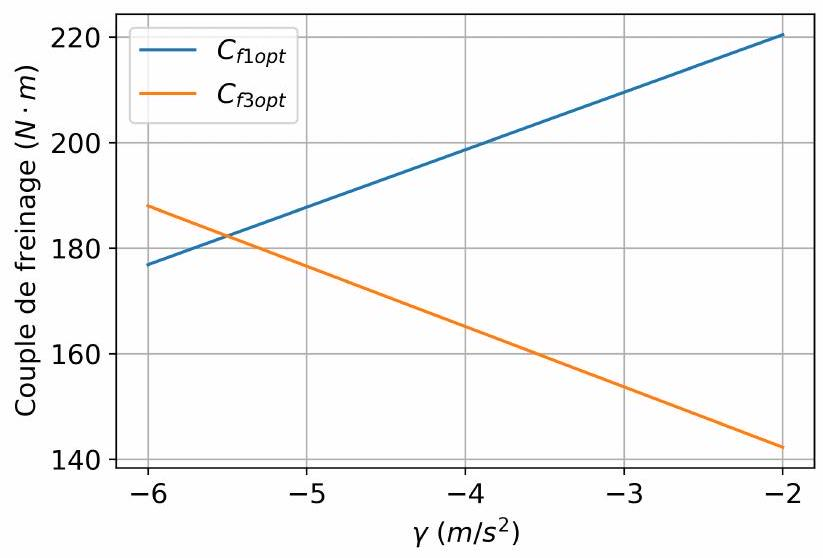
\includegraphics[width=0.8\textwidth]{2024_12_06_8b2ce2e701dae8972925g-11}
\caption{Couples de freinage optimaux en fonction de la décélération visée \label{fig6}}
\end{center}
\end{figure}

\question{Pour une décélération visée «dite d'urgence» conforme à l'exigence 210 de \(-4.5 \mathrm{~m} \cdot \mathrm{~s}^{-2}\), déterminer les couples de freinage optimaux à mettre en œuvre sur chacune des roues.}

\question{Conclure quant au système de freins installé sachant que les freins installés sur le G4e permettent d'envisager un couple de freinage maximum de \(250 \mathrm{~N} \cdot \mathrm{~m}\) pour une distance parcourue de 6 m .}

Le contrôle du freinage, assuré par le conducteur, est réalisé par l'action de ses mains sur chacune des poignées de frein. Le cycliste module ainsi l'intensité du couple de freinage sur chacune des roues au travers de son ressenti. Les couples de freinage peuvent donc s'en trouver non optimaux.

\question{Proposer une solution technologique de pilotage des freins qu'il serait possible d'intégrer pour optimiser les conditions de freinage.}


\section{Étude du capteur de couple}

Le groupe d'assistance dont est pourvu le vélo cargo assiste le cycliste en fonction du couple que celui-ci applique sur le pédalier. Ce groupe d'assistance comporte donc un capteur destiné à acquérir le couple appliqué par le cycliste sur le pédalier. Cette section vise à modéliser ce capteur et à en dimensionner certains éléments.\\

\begin{figure}[!htb]
\begin{center}
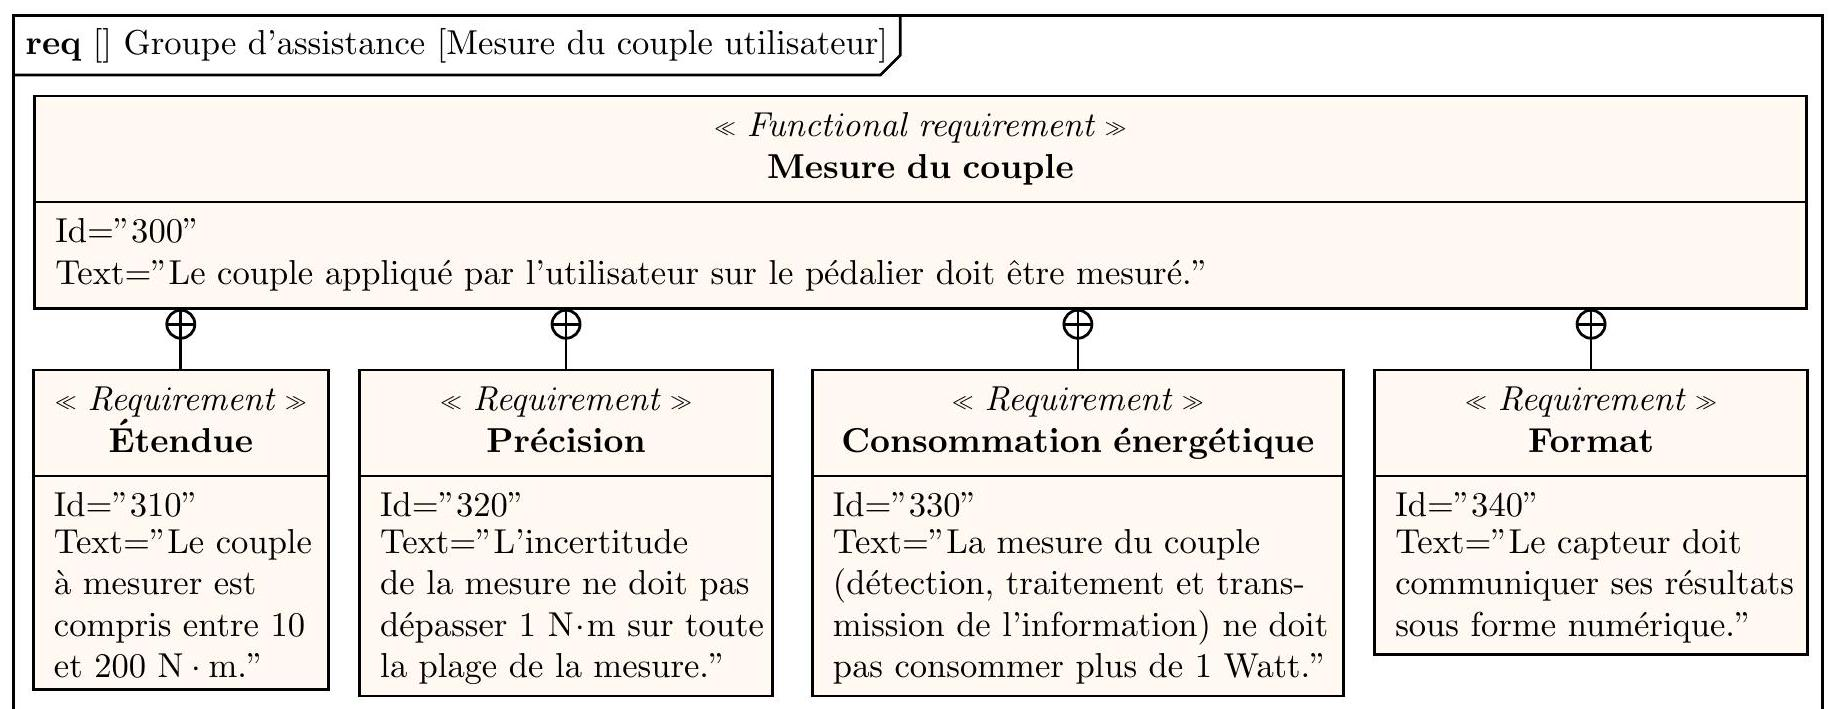
\includegraphics[width=0.8\textwidth]{2024_12_06_8b2ce2e701dae8972925g-12(1)}
\caption{Extrait du cahier des charges relatif à la mesure du couple appliqué par l'utilisateur sur le pédalier. \label{fig_41}}
\end{center}
\end{figure}

\subsection{Présentation du capteur}
Le capteur utilisé est composé d'un transducteur à reluctance variable (présenté ci-dessous), d'un circuit d'amplification et de détection d'amplitude (non étudié) et d'un convertisseur analogique numérique.

\begin{figure}[!htb]
\begin{center}
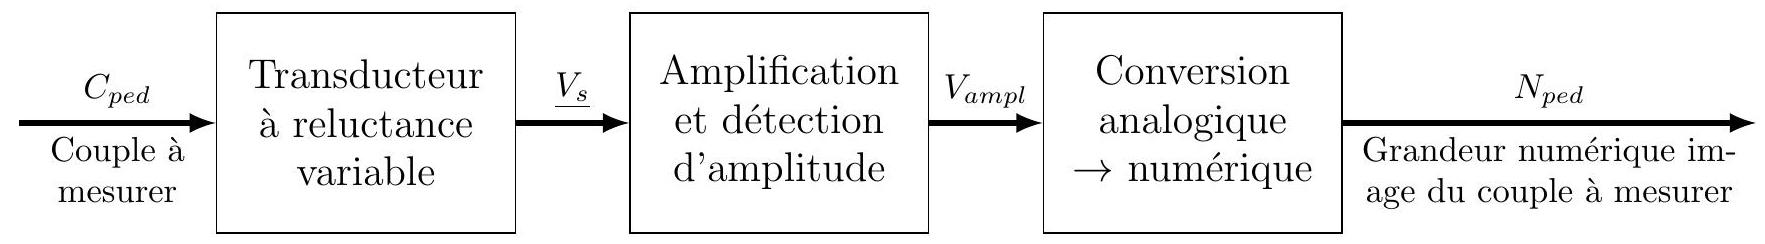
\includegraphics[width=0.8\textwidth]{2024_12_06_8b2ce2e701dae8972925g-12}
\caption{Architecture du capteur de couple \label{fig_42}}
\end{center}
\end{figure}

Constitution du transducteur à reluctance variable Un schéma de principe du transducteur à reluctance variable autour duquel est construit le capteur de couple étudié est donné figure \ref{fig_43}. Ce transducteur est constitué de quatre ensembles :

\begin{itemize}
  \item l'arbre A1 sur lequel est monté un anneau magnétique Am1,
  \item l'arbre A2 sur lequel sont montés les anneaux magnétiques Am21 et Am22,
  \item l'arbre de torsion At qui relie les arbres A1 et A2,
  \item un bâti (non représenté sur la figure 4.3). Les arbres A1 et A2 sont guidés en rotation par rapport à ce bâti. Les bobines de détection Bd et de compensation Bc sont solidaires du bâti.
\end{itemize}

Principe de la mesure Les bobines Bd et Bc sont alimentées par une source de tension sinusoïdale.

Le circuit magnétique constitué par la bobine de compensation et les anneaux magnétiques Am21 et Am22 est indéformable. Son inductance est donc indépendante du couple transmis (cette bobine sert à compenser la dérive en température).

Le circuit magnétique constitué par la bobine de détection et les anneaux magnétiques Am1 et Am21 se déforme en même temps que l'arbre de torsion. Cette déformation provoque une variation de l'inductance de la bobine de détection. Le transducteur est construit de telle sorte que cette variation d'inductance soit proportionnelle au couple à mesurer.

\begin{figure}[!htb]
\begin{center}
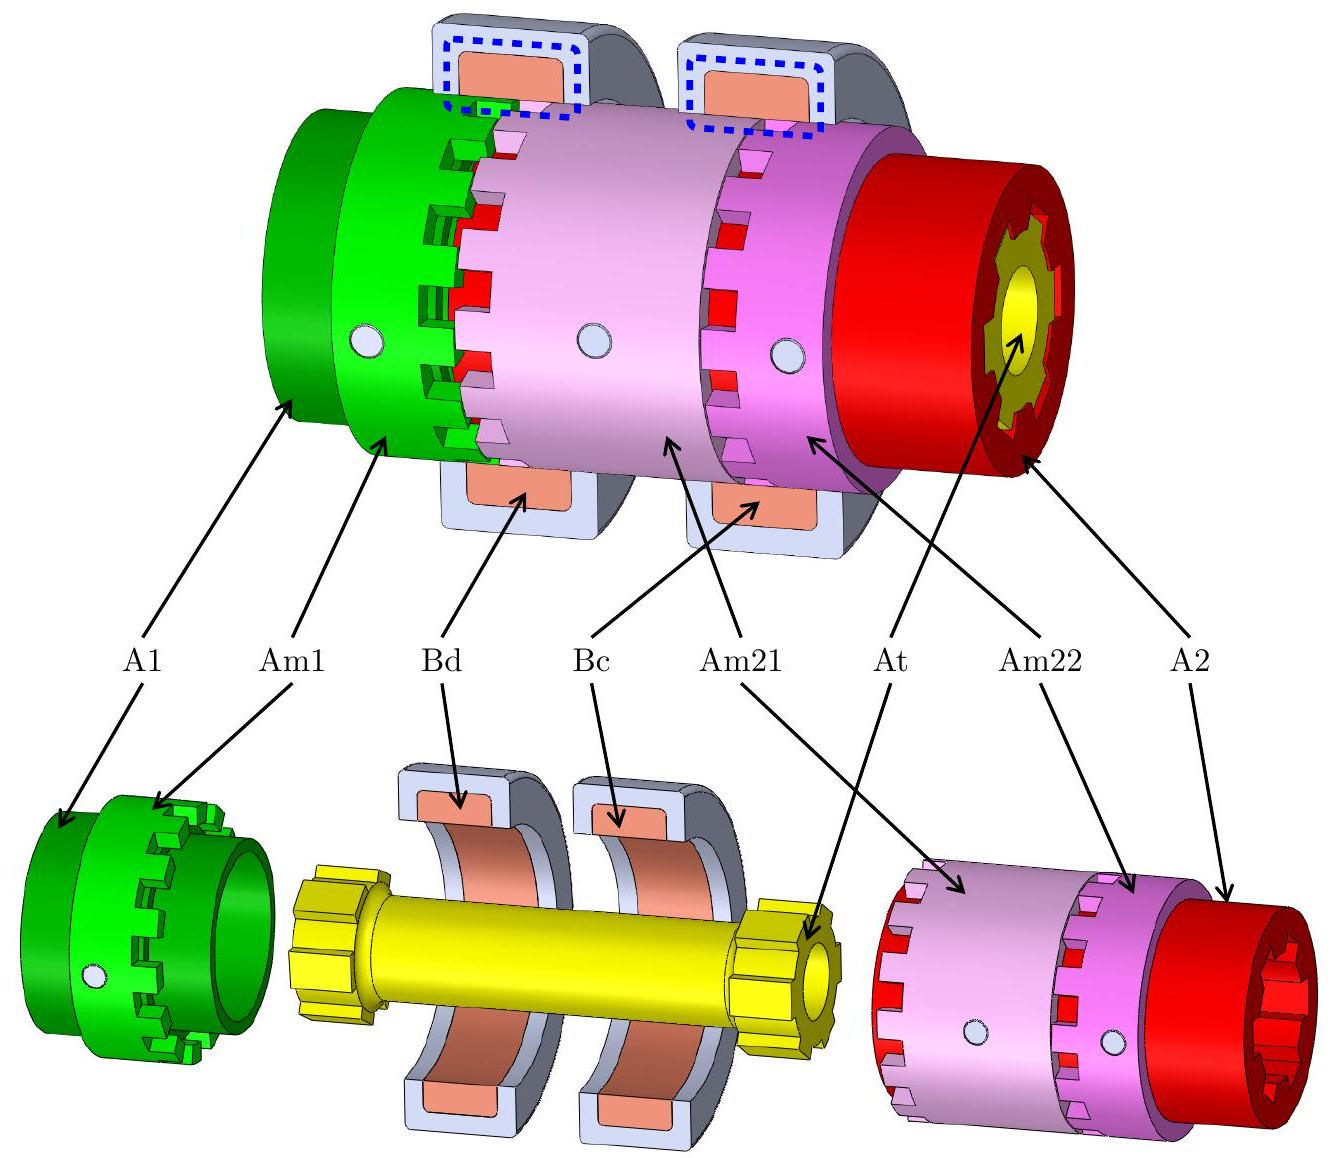
\includegraphics[width=0.8\textwidth]{2024_12_06_8b2ce2e701dae8972925g-13}
\caption{Principaux éléments du transducteur de couple \label{fig_43}}
\end{center}
\end{figure}


\subsection{Tension de sortie du transducteur}

\begin{obj}
\(\underline{\text { Exprimer la tension de sortie } v_{s} \text { du transducteur de couple en fonction de la variation d'inductance } \Delta L}\).
\end{obj}

Le transducteur de couple est modélisé par deux bobines d'inductances respectives \(L_{1}\) (bobine de compensation) et \(L_{1}+\Delta L\) (bobine de détection). La résistance de ces bobines n'est pas négligée. Ces bobines sont insérées dans le montage schématisé figure \ref{fig_44}. Les deux sources de tension sinusoïdales \(v_{1}\) et \(v_{2}\) ont même valeur moyenne, même amplitude et sont en opposition de phase. La différence de potentiel \(v_{s}\) entre les points \(A\) et \(B\) du schéma de la figure \ref{fig_44} constitue la tension de sortie du transducteur.

\paragraph*{Régime continu}
On étudie dans un premier temps le fonctionnement du capteur en régime continu.


\question{En supposant que l'amplitude \(A\) des tensions \(v_{1}\) et \(v_{2}\) est nulle, donner sans justification les valeurs :}
\begin{enumerate}
  \item de la tension \(v_{s}\),
  \item de la puissance débitée par chacune des deux sources de tension \(v_{1}\) et \(v_{2}\).
\end{enumerate}
\ifprof
\begin{corrige}

\end{corrige}
\else
\fi

\paragraph*{Régime alternatif} L'étude du régime continu a permis de montrer qu'il est possible de remplacer les deux sources de tension \(v_{1}\) et \(v_{2}\) par une unique de source de tension \(v_{12}=v_{1}-v_{2}\). Le transducteur fonctionnant en régime sinusoïdal forcé, on utilise les notations complexes des grandeurs électriques. À partir de la question 33, l'étude est menée sur la base du schéma de la figure \ref{fig_45}. Les valeurs numériques définies figure \ref{fig_44} sont conservées. La tension

$
\underline{V_{12}}=\sqrt{2} \cdot 2 \cdot A \cdot e^{j \cdot \omega \cdot t} \quad(\omega=2 \cdot \pi \cdot f)
$

est prise pour référence de phases.\\

\begin{figure}[!htb]
\begin{center}
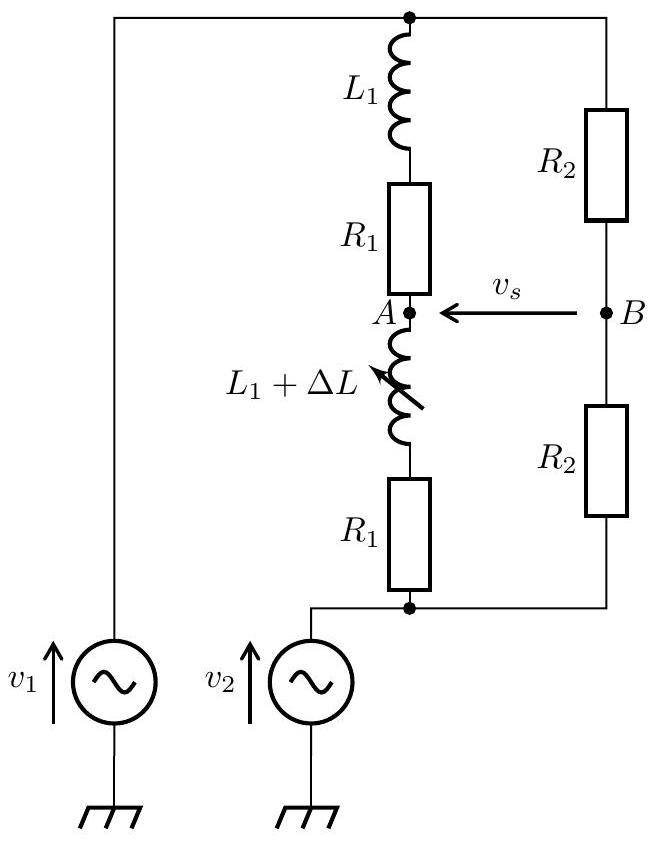
\includegraphics[width=0.8\textwidth]{2024_12_06_8b2ce2e701dae8972925g-14}
\caption{ Modèle électrique du transducteur de couple et grandeurs associées \label{fig_44}}
\end{center}
\end{figure}

$
\begin{aligned}
L_{1} & =5 \mathrm{mH} \\
-\Delta L_{\text{Max}} \leq & \Delta L \leq 0 \mathrm{mH} \text { avec }: \Delta L_{\text{Max}}=1 \mathrm{mH} \\
R_{1} & =5 \Omega \\
v_{1} & =\dfrac{E}{2}+\sqrt{2} \cdot A \cdot \cos (2 \cdot \pi \cdot f \cdot t) \\
v_{2} & =\dfrac{E}{2}-\sqrt{2} \cdot A \cdot \cos (2 \cdot \pi \cdot f \cdot t) \\
E & =24 \mathrm{~V} \\
A & =8 \mathrm{~V} \\
f & =20 \mathrm{kHz}
\end{aligned}
$

Figure \ref{fig_4_cargo}.4 - Modèle électrique du transducteur de couple et grandeurs associées\\

\begin{figure}[!htb]
\begin{center}
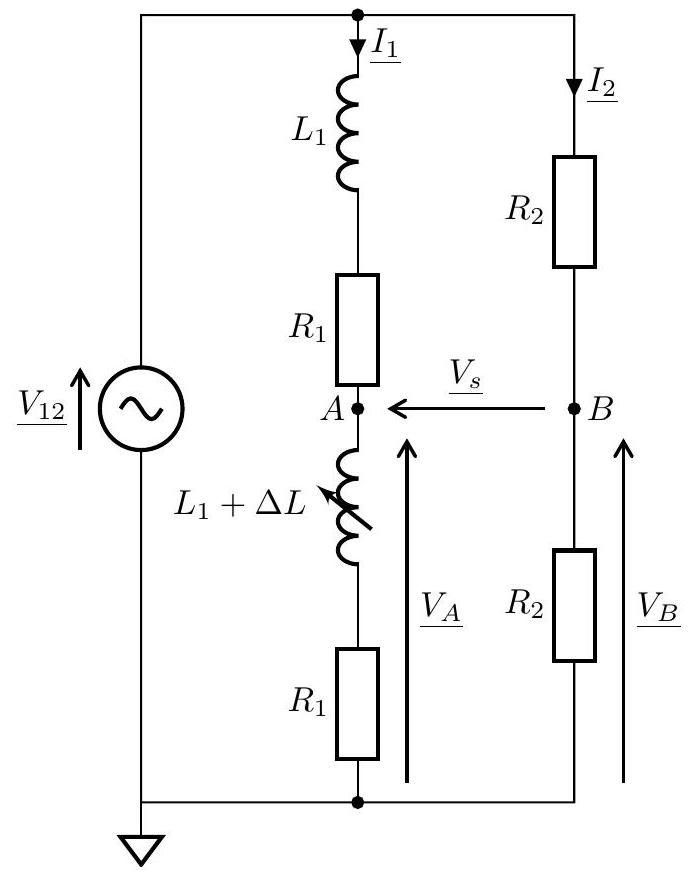
\includegraphics[width=.8\linewidth]{2024_12_06_8b2ce2e701dae8972925g-14(1)}
\caption{Modèle électrique du transducteur de couple en régime alternatif \label{fig10}}
\end{center}
\end{figure}

\question{Exprimer les tensions \(\underline{V_{A}}\) et \(\underline{V_{B}}\) en fonction de \(\underline{V_{12}}\) et des paramètres définis figure 4.5.}

\ifprof
\begin{corrige}

\end{corrige}

\else
Question 34 : En déduire les expressions des paramètres \(X_{v a r}, R_{t o t}\) et \(X_{t o t}\) tels que:

$
\underline{V_{S}}=\dfrac{j \cdot X_{v a r}}{2 \cdot\left(R_{t o t}+j \cdot X_{t o t}\right)} \cdot \underline{V_{12}}
$

Question 35 : Calculer la valeur de \(R_{t o t}\) ainsi que les valeurs extrémales de \(X_{t o t}\). Proposer alors une simplification de la grandeur \(\left|\underline{V_{S}} / \underline{V_{12}}\right|\).

Question 36 : Indiquer la condition que doivent satisfaire les grandeurs \(L_{1}\) et \(\Delta L\) afin de pouvoir considérer le transducteur linéaire.

\subsection{4.3 Consommation énergétique du transducteur}
\section{Objectif}
Dimensionner les résistances \(R_{2}\).\\
Rappel : le transducteur est étudié sur la base du modèle donné figure 4.5, les valeurs numériques relatives à ce modèle sont données figure 4.4.

Exigence de consommation Afin de respecter l'exigence 330 (figure 4.1), la puissance consommée par le transducteur ne doit pas dépasser 0.5 W .

Hypothèse supplémentaire L'étude de la consommation énergétique du transducteur est menée en supposant \(\Delta L=0 \mathrm{H}\).

Question 37 : Exprimer, en fonction de \(A\) et des éléments du schéma du transducteur, le courant efficace \(I_{1}\). Calculer sa valeur.

Question 38 : Exprimer la puissance \(P_{\text {trans }}\) absorbée par le transducteur en fonction de \(R_{1}, R_{2}\) et \(A\).\\
\(\square\) Question 39 : Déduire des questions précédentes la valeur minimale de \(R_{2}\) qui permet de limiter la puissance \(P_{\text {trans }}\) absorbée par le transducteur à 0.5 W .

\subsection{4.4 Dimensionnement du CAN}
\section{Objectif}
Estimer l'influence du convertisseur analogique \(\rightarrow\) numérique sur le respect de l'exigence de précision.

\section{Modélisation des éléments du capteur}
\begin{itemize}
  \item L'étude de transducteur de couple a permis d'établir que ce transducteur a un comportement linéaire. On l'assimile donc à un gain, noté \(K_{\text {trans }}\) tel que l'amplitude de la tension \(v_{s}\) en sortie du transducteur soit égale à \(K_{\text {trans }} \cdot C_{p e d}\) où \(C_{p e d}\) désigne le couple à mesurer et \(K_{\text {trans }}=6.2 \cdot 10^{-3} \mathrm{~V} /(\mathrm{N} \cdot \mathrm{m})\).
  \item L'étage d'amplification et de mesure d'amplitude est modélisé par un gain de valeur \(K_{a m p l}=4\).
\end{itemize}

Le modèle adopté pour la chaîne de traitement de l'information dans le capteur de couple est résumé par le diagramme de la figure 4.6.\\

\begin{figure}[!htb]
\begin{center}
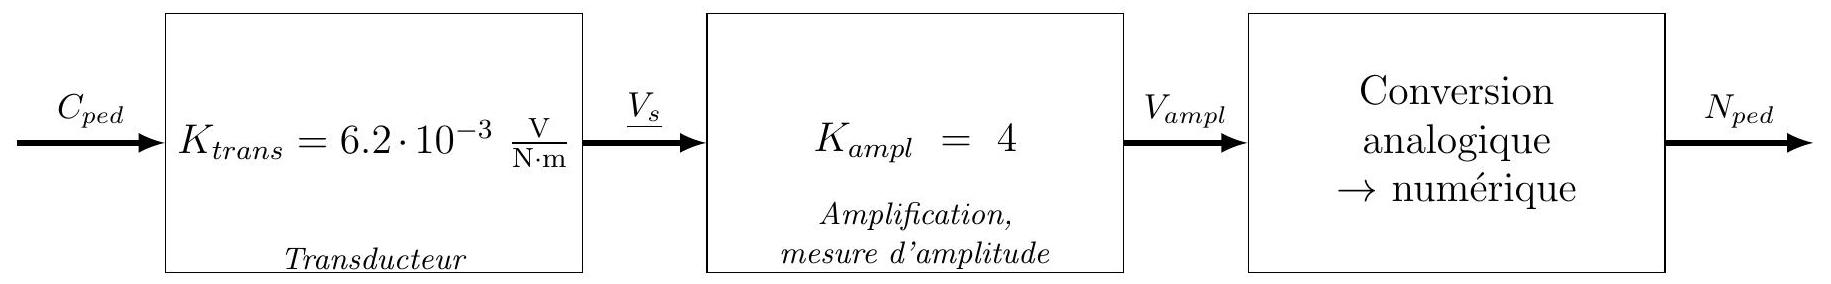
\includegraphics[width=0.8\textwidth]{2024_12_06_8b2ce2e701dae8972925g-15}
\caption{Chaîne de traitement de l'information dans le capteur de couple \label{fig11}}
\end{center}
\end{figure}

Convertisseur analogique \(\rightarrow\) numérique Le CAN utilisé dans le capteur présente les caractéristiques suivantes:

\begin{center}
\begin{tabular}{lcl}
Grandeur & Symbole & Valeur \\
\hline
Résolution & \(R\) & 16 bits \\
Tension de référence basse & \(V_{\text {ref- }}\) & 0 V \\
Tension de référence haute & \(V_{\text {reft }}\) & 5 V \\
\hline
\end{tabular}
\end{center}

Tableau 4.1 - Caractéristiques du CAN

Question 40 : Calculer l'incertitude introduite sur la mesure du couple \(C_{p e d}\) par la conversion analogique \(\rightarrow\) numérique. Comparer cette incertitude à celle tolérée par l'exigence de précision (exigence 320, figure 4.1) et conclure quant au dimensionnement du CAN.

\subsection{4.5 Durée de la conversion analogique \(\rightarrow\) numérique}
Le CAN utilisé pour la mesure du couple pédalier est un CAN à approximations successives. Ce CAN, dont l'architecture est présentée figure 4.7, réalise la conversion analogique \(\rightarrow\) numérique en suivant l'agorithme décrit figure 4.8. Le fonctionnement de ce CAN est cadencé sur le signal d'horloge SCLK. On admet que chaque opération (comparaison, affectation, ...) est réalisée en un coup d'horloge.\\

\begin{figure}[!htb]
\begin{center}
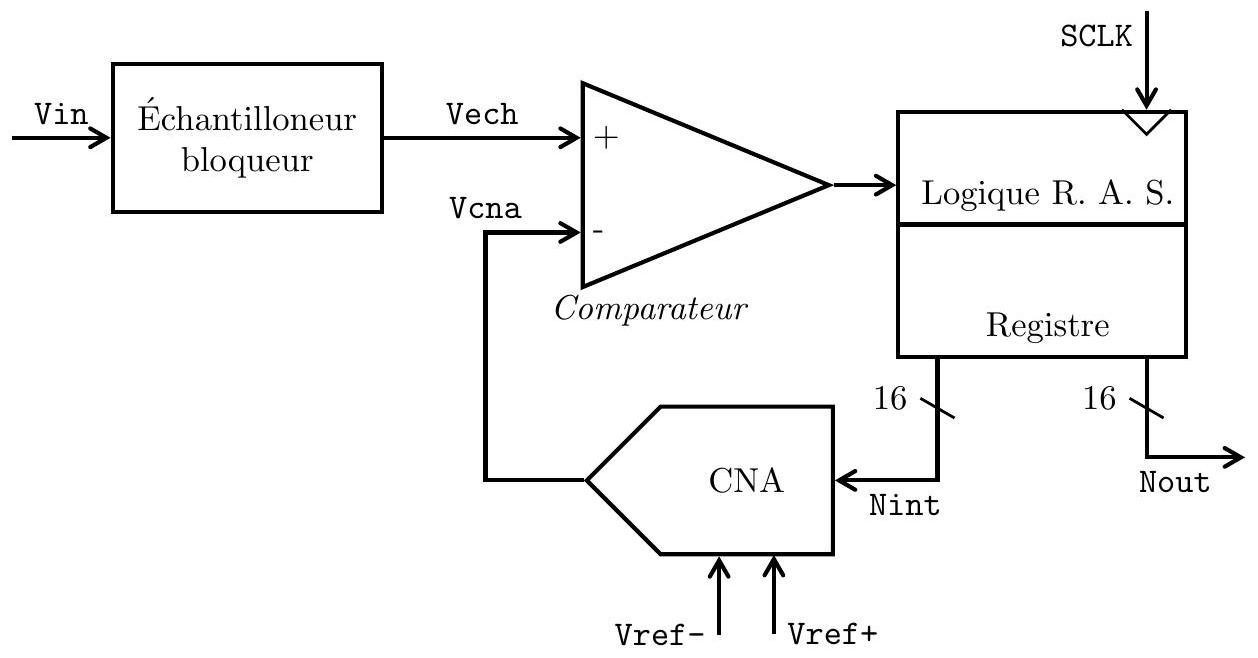
\includegraphics[width=0.8\textwidth]{2024_12_06_8b2ce2e701dae8972925g-16}

Le CNA a la même résolution et les mêmes tensions de référence que le CAN auquel il est intégré (voir tableau 4.1). La mise à 1 du bit de poids j dans le mot Nint incrémente la tension Vcna de

$
\dfrac{2^{j}}{2^{16}} \cdot(\text { Vref }+- \text { Vref }-)
$

Figure \ref{fig_4_cargo}.7 - Architecture d'un CAN à approximations successives

\begin{verbatim}
# Initialisation
Nint = 0000 0000 0000 0000 #Nint est codé en binaire naturel
j = 15
# Conversion par approximations successives
Tant que (j >= 0)
{
    Nint[j] = 1 #affecter 1 au bit de poids j de Nint
    Appliquer Nint en entrée du CNA
    Si (Vcna > Vech)
    {
            Nint[j] = 0 #Remettre le bit de poids j de Nint à 0
        }
        j = j-1 #passage au bit de poids inférieur
}
# Communication résultat
Nout = Nint
\end{verbatim}
\caption{Algorithme de conversion par approximations successives (les \# désignent les commentaires) \label{fig12}}
\end{center}
\end{figure}

Question 41 : Sur le document réponse C, pour les quatre premières itérations de la boucle Tant que,

\begin{enumerate}
  \item indiquer la valeur en binaire prise par Nint,
  \item tracer l'évolution de la tension Vcna\\
au moment de l'exécution de la ligne \(« j=j-1 \ldots\) dans le cas où la tension Vech vaut 4.0625 V .
\end{enumerate}

\fi
\question{Déterminer, en nombre de coups d'horloge, la durée que met le CAN à réaliser une conversion dans le cas le plus défavorable (cas où le nombre d'opérations est le plus élevé).}

\ifprof
\begin{corrige}

\end{corrige}

\else
Question 43 : Déduire de la question précédente la fréquence minimale du signal d'horloge \(f_{S C L K}\) qui permet de réaliser 20000 conversions par seconde.

\section{5 Modélisation de l'association \{ onduleur + machine synchrone \}}
\section{Objectif}
Modéliser le fonctionnement de l'association \{ Machine synchrone à fcem trapézoïdales + onduleur \}.\\
Le groupe d'assistance est animé par une machine synchrone triphasée dont les forces contre-électromotrices présentent une évolution temporelle trapézoïdale (figure 5.1). Du fait de son comportement analogue à une machine à courant continu, l'association \{ machine à fcem trapézoïdales + onduleur \} porte la désignation commerciale de «machine à courant continu sans balais» (de l'anglais BLDC pour «BrushLess Direct Courant motor»). Cette partie vise à modéliser le fonctionnement de cette association machine - modulateur.

Les grandeurs et notations utiles dans la suite de cette partie sont définies dans le tableau 5.1 ainsi que sur les figures 5.2 et 5.3. La figure 5.3 détaille l'architecture de l'association onduleur + machine. L'onduleur est piloté de telle sorte que les courants \(i_{1}, i_{2}\) et \(i_{3}\) absorbés par chaque phase suivent le profil idéal défini figure 5.2.\\

\begin{figure}[!htb]
\begin{center}
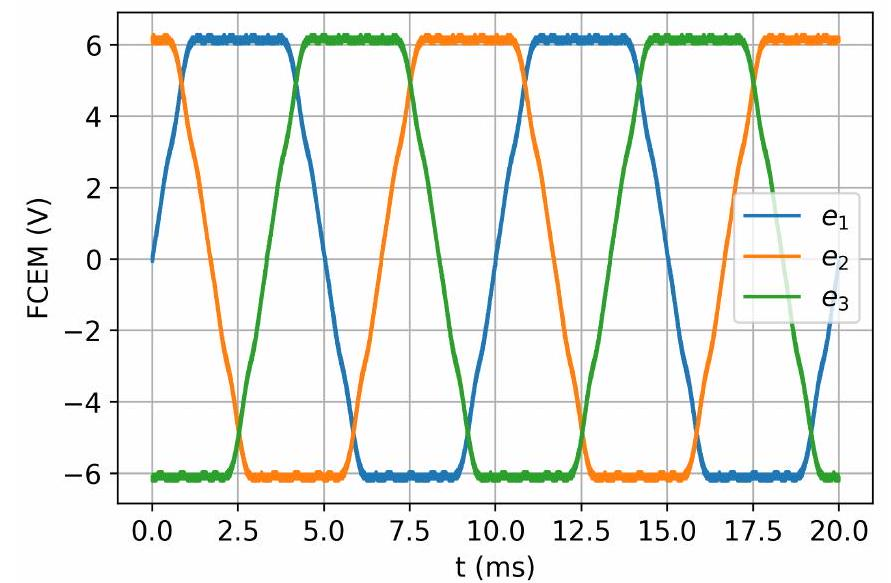
\includegraphics[width=0.8\textwidth]{2024_12_06_8b2ce2e701dae8972925g-17}

\begin{center}
\begin{tabular}{lll}
Grandeur & Symbole & Valeur \\
\hline
Nombre de paires de pôles & \(p\) & 2 \\
par phase &  &  \\
Vitesse de rotation & \(\omega_{m}\) &  \\
Phase électrique & \(\theta_{e}\) &  \\
\hline
\end{tabular}
\end{center}

Tableau 5.1 - Données et notations relatives à la machine étudiée

Figure \ref{fig_5_cargo}.1 - Forces électromotrices induites lors de la mise en rotation de la machine

Question 44 : À partir de la figure 5.1, calculer, dans les unités du système international, la constante \(k_{\phi}\) telle que \(E_{\max }=k_{\phi} \cdot \omega_{m}\).

\subsection{5.1 Expression du couple électromagnétique}
On note \(P_{\text {emg }}\) la puissance électromagnétique instantanée délivrée par la machine.

Question 45 : Exprimer la puissance \(P_{e m g}\) quelle que soit la valeur de \(\theta_{e}\) en fonction des tensions et courants définis figure 5.3.

Question 46 : Dans le cas particulier où \(\theta_{e}\) est compris entre 30 et \(90^{\circ}\), exprimer \(P_{e m g}\) en fonction de \(E_{\max }\) et \(i_{10}\).

Question 47 : Déterminer la condition portant sur les courants \(i_{10}, i_{20}\) et \(i_{30}\) qui permet de rendre constante la puissance électromagnétique \(P_{e m g}\) délivrée par la machine.

Question 48 : En supposant que la puissance \(P_{e m g}\) est constante, montrer que le couple électromagnétique délivré par la machine est proportionnel au courant \(i_{o n d}\) débité par l'onduleur : \(C_{m}=K_{m} \cdot i_{\text {ond }}\). Déterminer l'expression de \(K_{m}\).

\subsection{5.2 Acquisition du courant}
L'asservissement du courant absorbé par la machine est réalisé en appliquant une commande de type MLI (modulation de largeur d'impulsion) sur les transistors. Les transistors pilotés évoluent en fonction de la phase

Phase 1\\
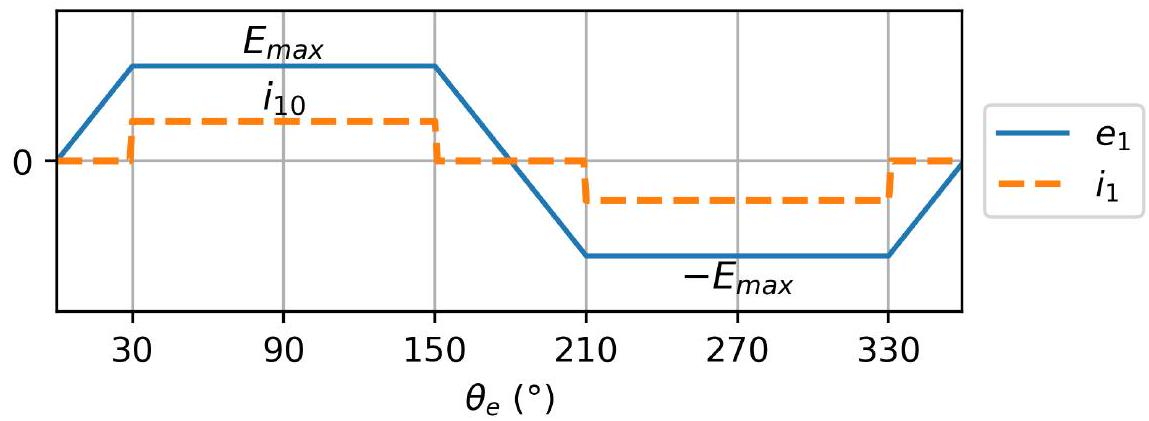
\includegraphics[width=.8\linewidth]{2024_12_06_8b2ce2e701dae8972925g-18}

Phase 2\\
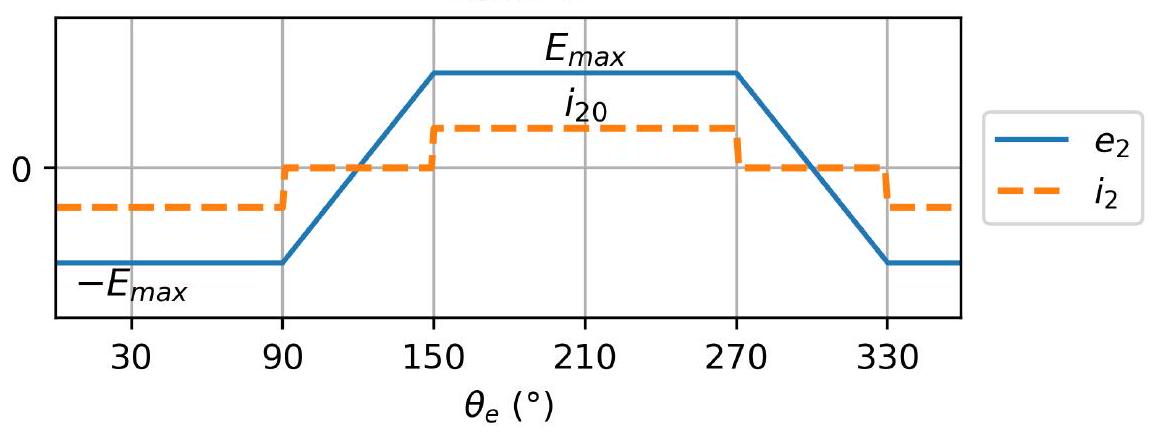
\includegraphics[width=.8\linewidth]{2024_12_06_8b2ce2e701dae8972925g-18(2)}

Phase 3\\
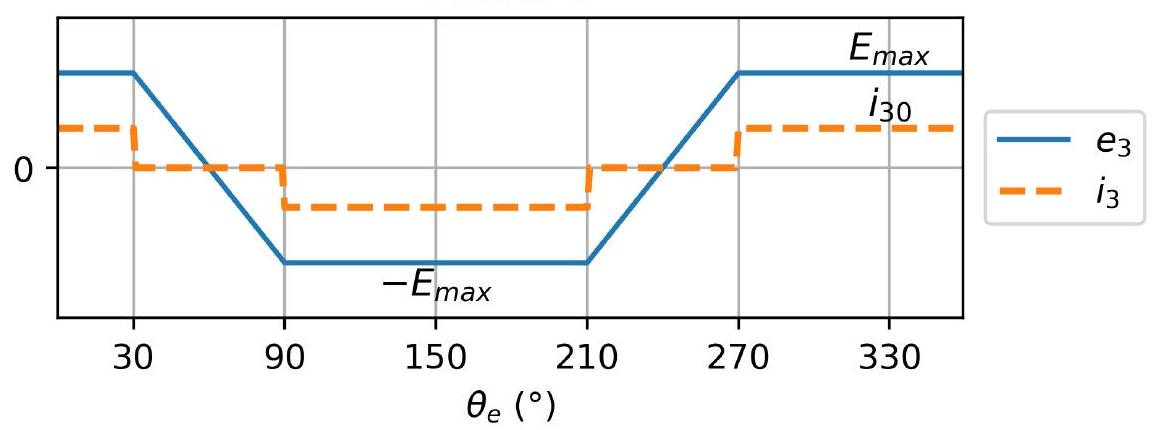
\includegraphics[width=.8\linewidth]{2024_12_06_8b2ce2e701dae8972925g-18(1)}

FIGURE 5.2 - FCEM et courants idéaux dans chaque phase de la machine\\
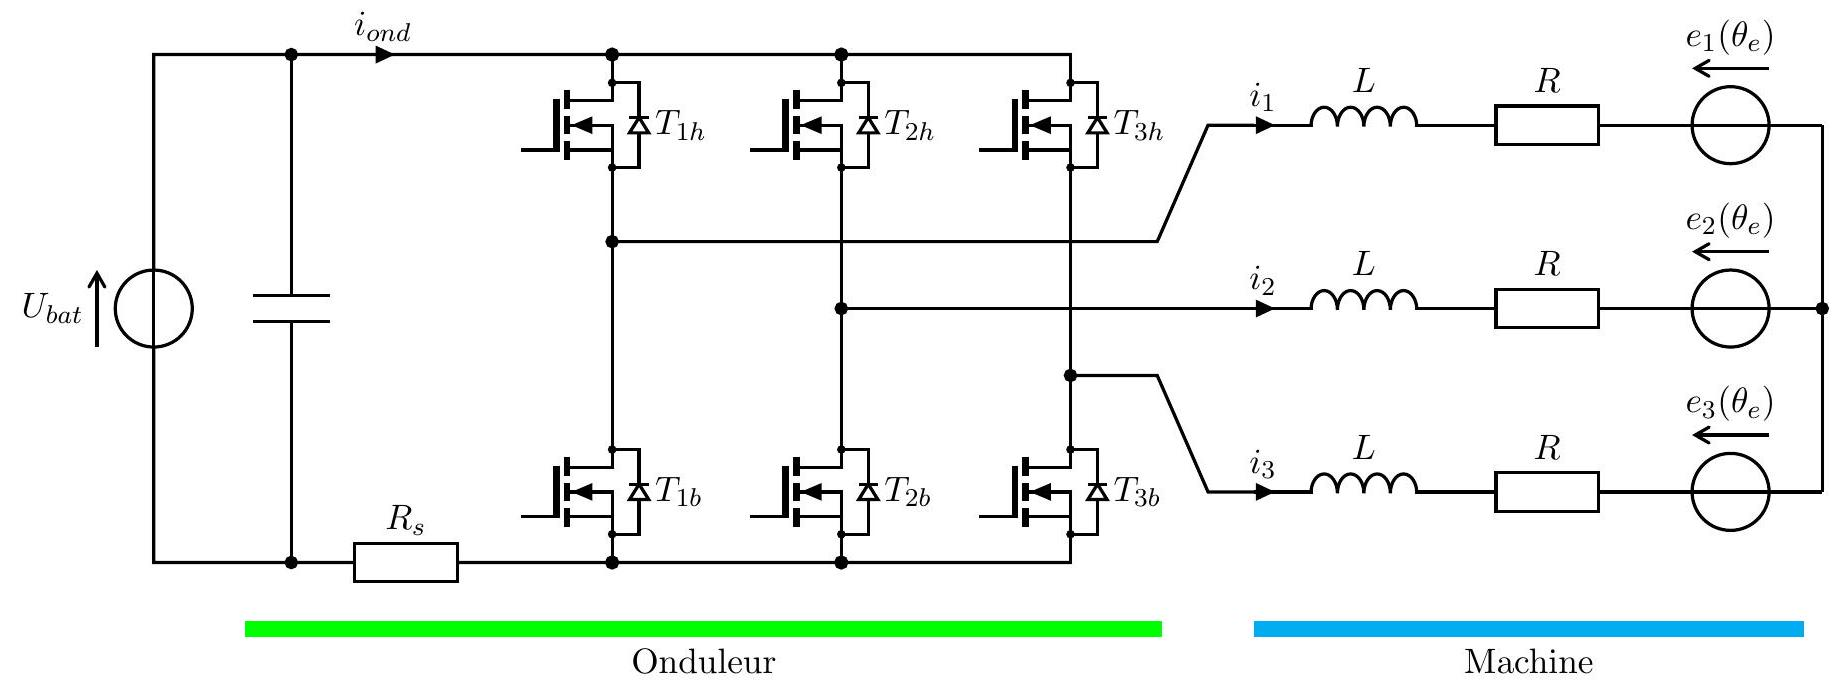
\includegraphics[width=.8\linewidth]{2024_12_06_8b2ce2e701dae8972925g-18(3)}
\caption{Machine synchrone à FEM trapézoïdale et modulateur associé\\ \label{fig13}}
\end{center}
\end{figure}
électrique \(\theta_{e}\). La résistance \(R_{s}\) (figure 5.3) est un shunt de \(3 \mathrm{~m} \Omega\) utilisé pour l'acquisition du courant absorbé par la machine.

Séquence de commande des transistors On s'intéresse au cas où \(\theta_{e}\) est compris entre 30 et \(90^{\circ}\). Au cours de cette phase, l'onduleur est piloté de la manière suivante :

\begin{itemize}
  \item les transistors \(T_{3 b}\) et \(T_{3 h}\) sont constamment bloqués,
  \item le transistor \(T_{2 b}\) est constamment saturé,
  \item le transistor \(T_{1 h}\) est piloté de manière périodique. En notant \(T\) la période de découpage et \(\alpha\) le rapport cyclique de découpage, ce transistor est piloté de la manière suivante :
  \item \(T_{1 h}\) est saturé pour \(t \in[0, \alpha \cdot T[\)
  \item \(T_{1 h}\) est bloqué pour \(t \in[\alpha \cdot T, T[\)
\end{itemize}

La période de découpage \(T\) est choisie beaucoup plus petite que la période des FCEM.

Question 49 : Sur le document réponse D, surligner la maille dans laquelle circule un courant au cours de chacun des deux temps de la période de découpage.

Question 50 : Tracer alors l'évolution temporelle de la chute de tension aux bornes du shunt \(R_{s}\) au cours d'une période de découpage. Indiquer la condition à satisfaire pour réaliser l'acquisition du courant absorbé par la machine.

\section{6 Asservissement du couple délivré par le groupe d'assistance}
L'architecture du groupe d'assistance dont est pourvu le vélo est présentée figure 6.3. Ce groupe d'assistance ajoute au couple \(C_{p c}\) appliqué par le cycliste sur le pédalier un couple \(C_{p m}\) délivré par la motorisation. Ce système est asservi de telle sorte que le couple \(C_{p m}\) appliqué par la motorisation est proportionnel au couple \(C_{p c}\) fourni par le cycliste : \(C_{p m}=K_{a s} \cdot C_{p c}\) (le couple \(C_{p m}\) sature à \(90 \mathrm{~N} \cdot \mathrm{~m}\) ). Le cycliste peut faire varier le niveau d'assistance entre 0 (groupe d'assistance désactivé) et 4 (assistance maximale). Chaque niveau d'assistance correspond à une valeur du coefficient d'assistance \(K_{a s}\) (figure 6.1).

Cahier des charges de l'asservissement en couple Les spécifications relatives à l'asservissement du couple appliqué par le groupe d'assistance au niveau de l'axe du pédalier sont données figure 6.2.\\

\begin{figure}[!htb]
\begin{center}
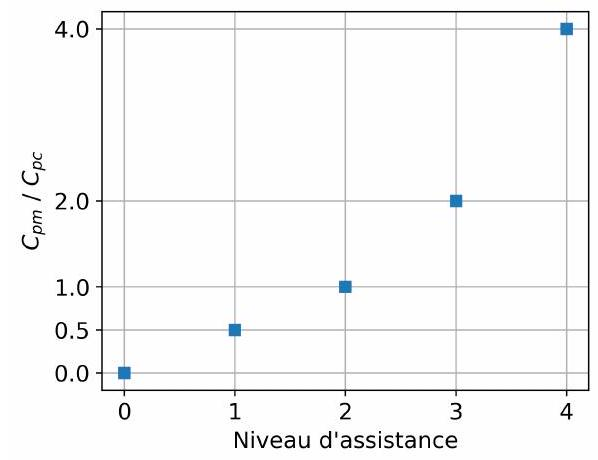
\includegraphics[width=0.8\textwidth]{2024_12_06_8b2ce2e701dae8972925g-20}
\caption{Évolution du coefficient d'assistance \(K_{a s}\) en fonction du niveau d'assistance\\ \label{fig14}}
\end{center}
\end{figure}

\begin{figure}[!htb]
\begin{center}
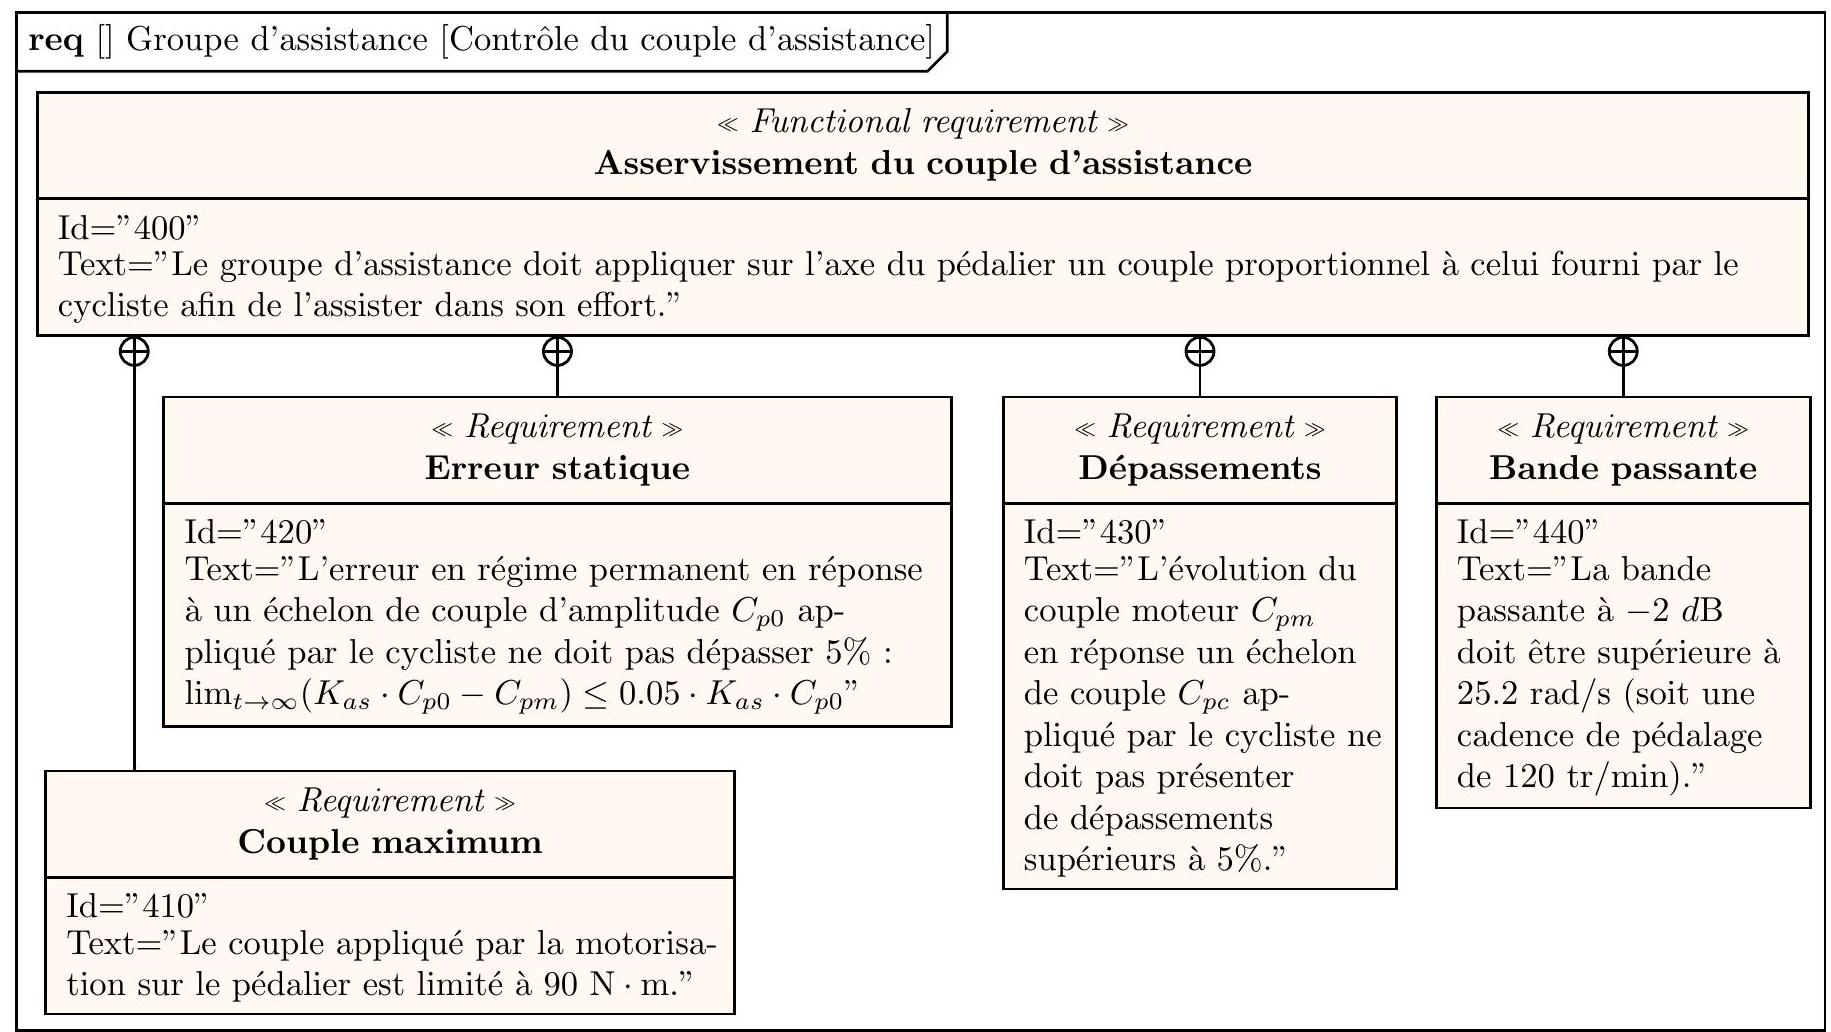
\includegraphics[width=0.8\textwidth]{2024_12_06_8b2ce2e701dae8972925g-20(1)}
\caption{Extrait du cahier des charges relatif au contrôle du couple d'assistance \label{fig15}}
\end{center}
\end{figure}

\subsection{6.1 Modélisation de l'asservissement du couple \(C_{p m}\)}
L'asservissement du couple délivré par le groupe d'assistance est modélisé sous la forme du schéma-bloc donné figure 6.4.

\section{Notations et hypothèses}
\begin{itemize}
  \item \(p\) désigne la variable de Laplace, la transformée de Laplace d'une fonction du temps \(f(t)\) est notée \(F(p)\).
  \item Les conditions de Heaviside sont supposées satisfaites.
  \item Les grandeurs introduites sur le schéma de la figure 6.4 sont recensées dans le tableau 6.1.\\

\begin{figure}[!htb]
\begin{center}
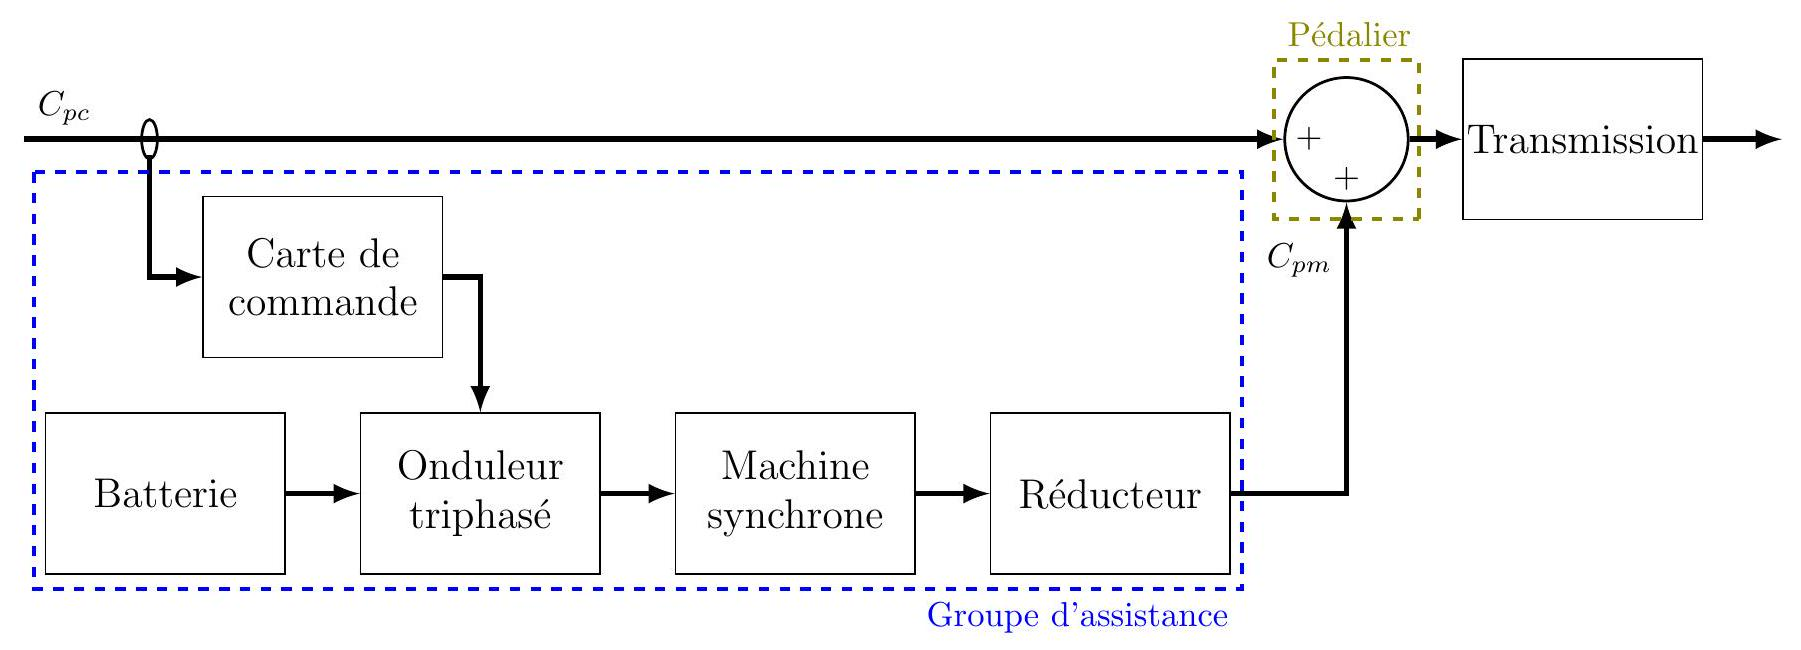
\includegraphics[width=0.8\textwidth]{2024_12_06_8b2ce2e701dae8972925g-21(1)}
\end{itemize}
\caption{Schéma d'architecture du groupe d'assistance\\ \label{fig16}}
\end{center}
\end{figure}

\begin{figure}[!htb]
\begin{center}
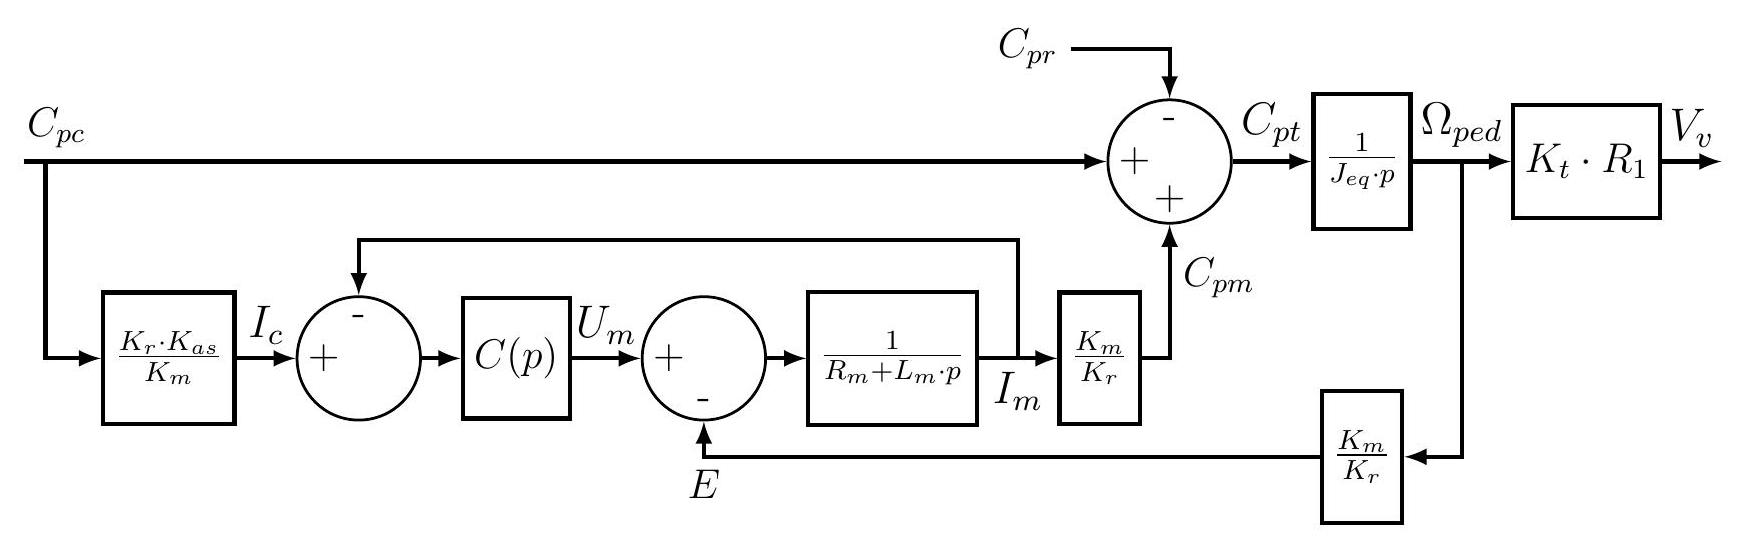
\includegraphics[width=0.8\textwidth]{2024_12_06_8b2ce2e701dae8972925g-21}
\caption{Schéma-bloc de l'asservissement du couple appliqué par le groupe d'assistance sur l'axe du pédalier \label{fig17}}
\end{center}
\end{figure}

\begin{center}
\begin{tabular}{clcc}
 & Grandeur & Symbole & Valeur \\
\hline
 & Coefficient d'assistance & \(K_{a s}\) &  \\
 & Fonction de transfert du correcteur & \(C(p)\) &  \\
\hline
Grandeurs & Rapport de transmission du réducteur du groupe d'assistance & \(K_{r}\) &  \\
mécaniques & Moment d'inertie de tout l'ensemble en mouvement ramené & \(J_{e q}\) &  \\
 & sur l'axe du pédalier &  &  \\
 & Rapport de transmission du pédalier à la roue & \(K_{t}\) &  \\
 & Rayon de la roue arrière & \(R_{1}\) &  \\
 & Couple appliqué par le cycliste sur le pédalier & \(C_{p c}(p)\) &  \\
 & Couple appliqué par la motorisation sur le pédalier & \(C_{p m}(p)\) &  \\
 & Couple résistant ramené sur l'axe du pédalier & \(C_{p r}(p)\) &  \\
 & Vitesse de rotation du pédalier & \(\Omega_{p e d}(p)\) &  \\
 & Vitesse de déplacement du vélo & \(V_{v}(p)\) &  \\
 & Masse de l'ensemble en mouvement & \(m_{T}\) &  \\
\hline
Machine & \(K_{m}\) & \(4 \cdot 10^{-2} \mathrm{~N} \cdot \mathrm{~m} / \mathrm{A}=\) &  \\
 & Constante de couplage &  & \(4 \cdot 10^{-2} \mathrm{~V} \cdot \mathrm{~s} / \mathrm{rad}\) \\
 &  & \(R_{m}\) & \(0.1 \Omega\) \\
 & Résistance d'induit & \(L_{m}\) & \(7 \cdot 10^{-4} \mathrm{H}\) \\
 & Inductance d'induit & \(E(p)\) &  \\
 & Force contre-électromotrice & \(U_{m}(p)\) &  \\
 & Tension d'induit &  &  \\
\hline
\end{tabular}
\end{center}

Tableau 6.1 - Grandeurs intervenant dans le schéma-bloc de la figure 6.4

Énergies cinétiques et inertie équivalente Au cours de son mouvement, le vélo accumule de l'énergie cinétique :

\begin{itemize}
  \item de par son mouvement de translation par rapport au sol,
  \item du fait des rotations par rapport à son cadre de certains éléments composent le vélo (roues, rotor du moteur, partie mobiles du réducteur, pédalier).\\
On admet que l'énergie cinétique accumulée par le mouvement de translation du vélo par rapport au sol est très grande devant l'énergie cinétique accumulée par les mouvements de rotation.
\end{itemize}

Question 51 : Déterminer l'expression du moment d'inertie équivalent \(J_{e q}\) de l'ensemble du vélo ramené sur l'axe du pédalier en fonction de \(m_{T}, R_{1}\) et \(K_{t}\).

\subsection{6.2 Simplification du modèle}
Le schéma-blocs donné figure 6.4 peut se mettre sous la forme du schéma simplifié donné figure 6.5 ci-dessous.\\

\begin{figure}[!htb]
\begin{center}
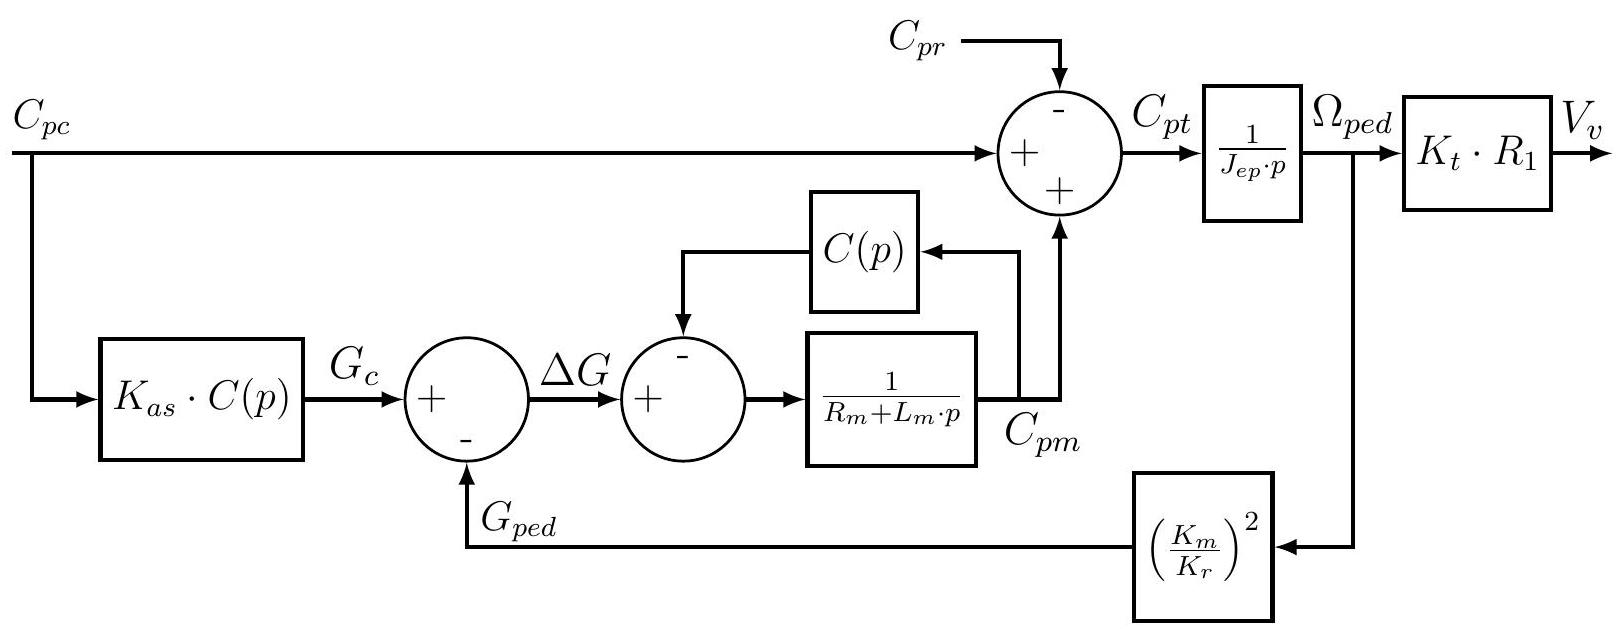
\includegraphics[width=0.8\textwidth]{2024_12_06_8b2ce2e701dae8972925g-22}
\caption{Schéma-bloc simplifié de l'asservissement du couple d'assistance \label{fig18}}
\end{center}
\end{figure}

Question 52 : À partir du schéma-bloc donné figure 6.4, déterminer la dimension de \(C(p)\). Justifier alors que les grandeurs \(G_{c}\) et \(G_{p e d}\) sont homogènes.

\fi
\question{Déterminer la fonction de transfert}

\ifprof
\begin{corrige}

\end{corrige}

\else
$
H_{G}(p)=\dfrac{C_{p m}(p)}{\Delta G(p)}
$

en fonction de \(C(p), R_{m}\) et \(L_{m}\).

\fi
\question{Déterminer l'expression de \(\Delta G(p)\) en fonction de \(C_{p c}(p), C_{p m}(p)\) et \(C_{p r}(p)\).}

\ifprof
\begin{corrige}

\end{corrige}

\else
\fi

\subsection{6.3 Correction proportionnelle (P)}
\section{Objectif}
Évaluer le respect des exigences dans le cas d'une correction proportionnelle.\\
On opte dans un premier temps pour une correction proportionnelle : \(C(p)=K_{c}\).\\
Question 55 : En supposant \(C_{p r}=0\), déterminer l'expression de la fonction de transfert :

$
H_{a s}(p)=\left.\dfrac{C_{p m}(p)}{C_{p c}(p)}\right|_{C_{p r}=0}
$

en fonction des grandeurs constantes définies dans le tableau 6.1.

Question 56 : Montrer alors que la correction proportionnelle ne permet pas de satisfaire l'exigence 420 portant sur l'erreur statique.

\subsection{6.4 Correction proportionnelle intégrale (PI)}
\section{Objectif}
Dimensionner un correcteur proportionnel intégral permettant de satisfaire le cahier des charges.\\
On évalue désormais le comportement de l'asservissement du couple d'assistance dans le cas d'une correction proportionnelle-intégrale :

$
C(p)=K_{c} \dfrac{1+T_{i} \cdot p}{T_{i} \cdot p}
$

Avec ce correcteur, la fonction de transfert \(H_{a s}(p)\) devient :

$
H_{a s}(p)=\dfrac{K_{a s} \cdot\left(K_{r}\right)^{2} \cdot J_{e q} \cdot K_{c}-\left(K_{m}\right)^{2} \cdot T_{i}+K_{a s} \cdot\left(K_{r}\right)^{2} \cdot J_{e q} \cdot K_{c} \cdot T_{i} \cdot p}{K_{c} \cdot\left(K_{r}\right)^{2} \cdot J_{e q}+\left(K_{m}\right)^{2} \cdot T_{i}+\left(K_{r}\right)^{2} \cdot J_{e q} \cdot T_{i} \cdot\left[R_{m}+K_{c}\right] \cdot p+\left(K_{r}\right)^{2} \cdot J_{e q} \cdot L_{m} \cdot T_{i} \cdot p^{2}}
$

Exigence de précision Le respect de l'exigence 420 impose :

$
\dfrac{K_{c}}{T_{i}} \geq \dfrac{100+95 \cdot K_{a s}}{5 \cdot K_{a s}} \cdot \dfrac{\left(K_{m}\right)^{2}}{K_{r} \cdot J_{e q}} \text { soit : } \quad \dfrac{K_{c}}{T_{i}} \geq 12.3 \cdot 10^{-3} \dfrac{\mathrm{~V}}{\mathrm{~A} \cdot \mathrm{~s}} \quad \text { pour } K_{a s}=0.5 \text { (cas le plus sévère) }
$

Exigence de bande passante Afin de respecter l'exigence 440 portant sur la bande passante de l'asservissement, on impose \(\omega_{0}=252 \mathrm{rad} / \mathrm{s}\).

Question 57 : Exprimer le dénominateur de \(H_{a s}\) sous forme canonique et en déduire l'expression de sa pulsation propre \(\omega_{0}\).

Question 58 : Déterminer la valeur du rapport \(K_{c} / T_{i}\) qui permet d'obtenir \(\omega_{0}=252 \mathrm{rd} / \mathrm{s}\).

Exigence portant sur les dépassements Le concepteur a choisi de régler le coefficient d'amortissement \(z\) à 1 ce qui conduit aux valeurs suivantes :

$
K_{c} \approx 0.253 \mathrm{~V} / \mathrm{A} \quad \text { et } \quad T_{i} \approx 5.69 \cdot 10^{-3} \mathrm{~s}
$

Simulation Le fonctionnement de l'asservissement du couple d'assistance est simulé pour \(K_{a s}=0.5\) avec les valeurs de \(K_{c}\) et \(T_{i}\) déterminées précédemment. De cette simulation sont extraits :

\begin{itemize}
  \item l'évolution du couple \(C_{p m}\) en réponse à un échelon de couple \(C_{p c}\) (figure 6.6),
  \item le diagramme de Bode du rapport \(C_{p m} / C_{p c}\) (figure 6.7).
\end{itemize}

Question 59 : Au regard du diagramme de Bode de la figure 6.7, proposer une forme simplifiée pour la fonction de transfert \(H_{a s}\).

Question 60 : À partir des figures 6.6 et 6.7, conclure quant au respect des exigences 420,430 et 440 du diagramme des exigences de la figure 6.2.

Fin du sujet.\\

\begin{figure}[!htb]
\begin{center}
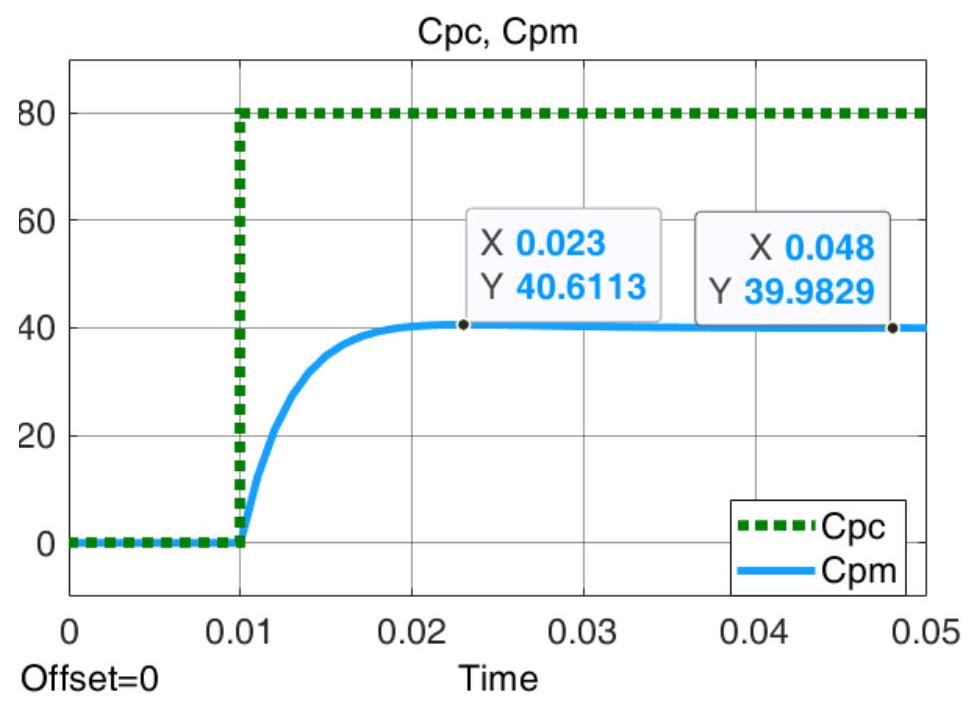
\includegraphics[width=0.8\textwidth]{2024_12_06_8b2ce2e701dae8972925g-24}
\caption{Évolution du couple d'assistance \(C_{p m}\) pour \(K_{a s}=0.5\) en réponse à un échelon d'amplitude \(80 \mathrm{~N} \cdot \mathrm{~m}\) \(\operatorname{sur} C_{p c}\)\\ \label{fig19}}
\end{center}
\end{figure}

\begin{figure}[!htb]
\begin{center}
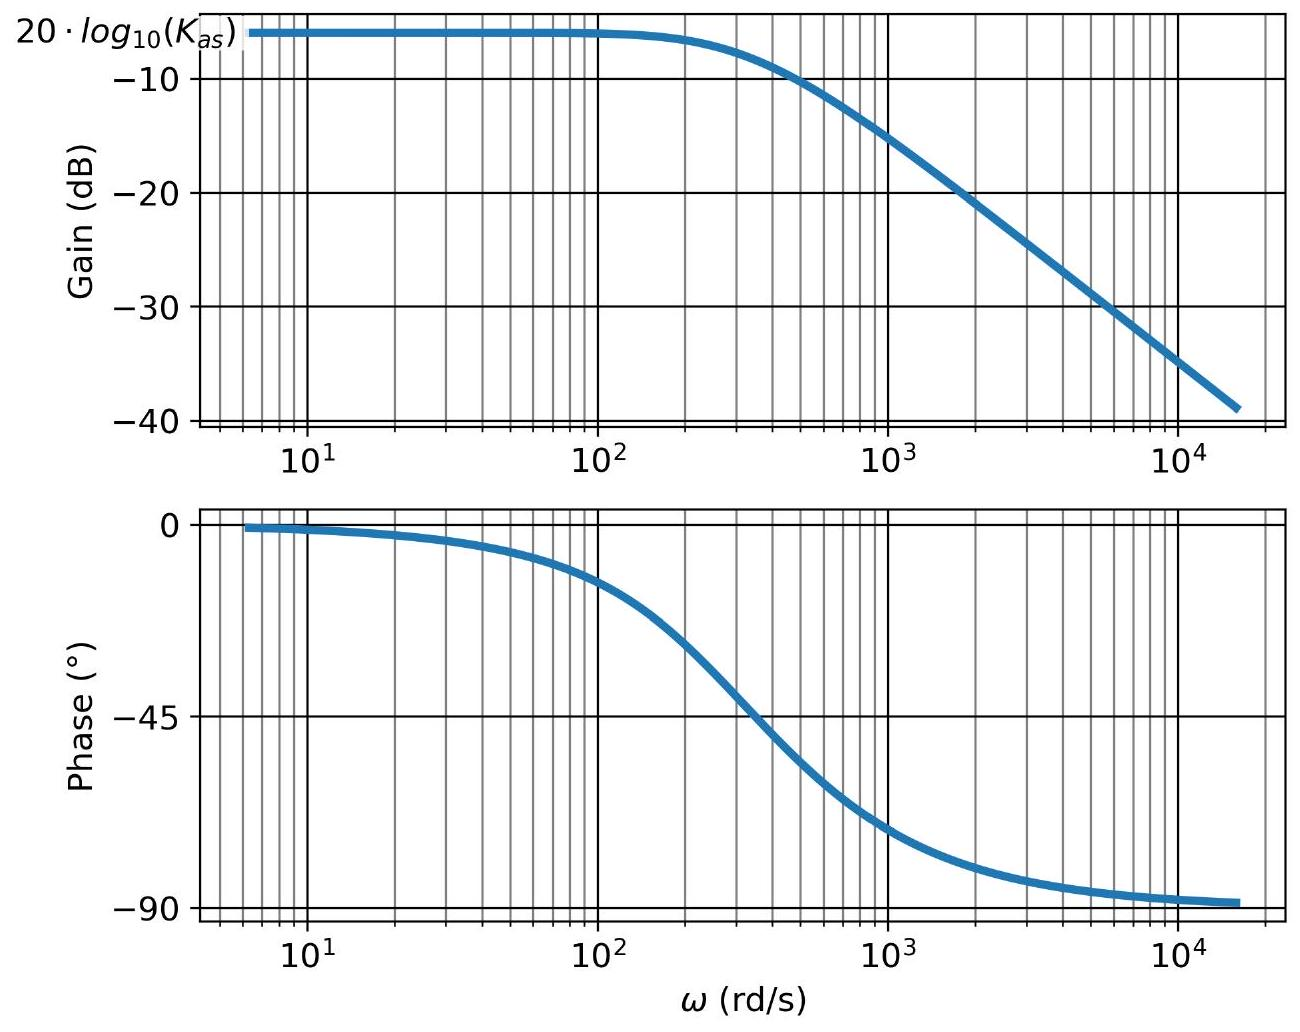
\includegraphics[width=0.8\textwidth]{2024_12_06_8b2ce2e701dae8972925g-24(1)}
\caption{Diagramme de Bode de la fonction de transfert \(H_{a s}(p)\) pour \(K_{a s}=0.5\) \label{fig20}}
\end{center}
\end{figure}

\section{Document réponse}
DR A : Schéma cinématique - Question 3\\
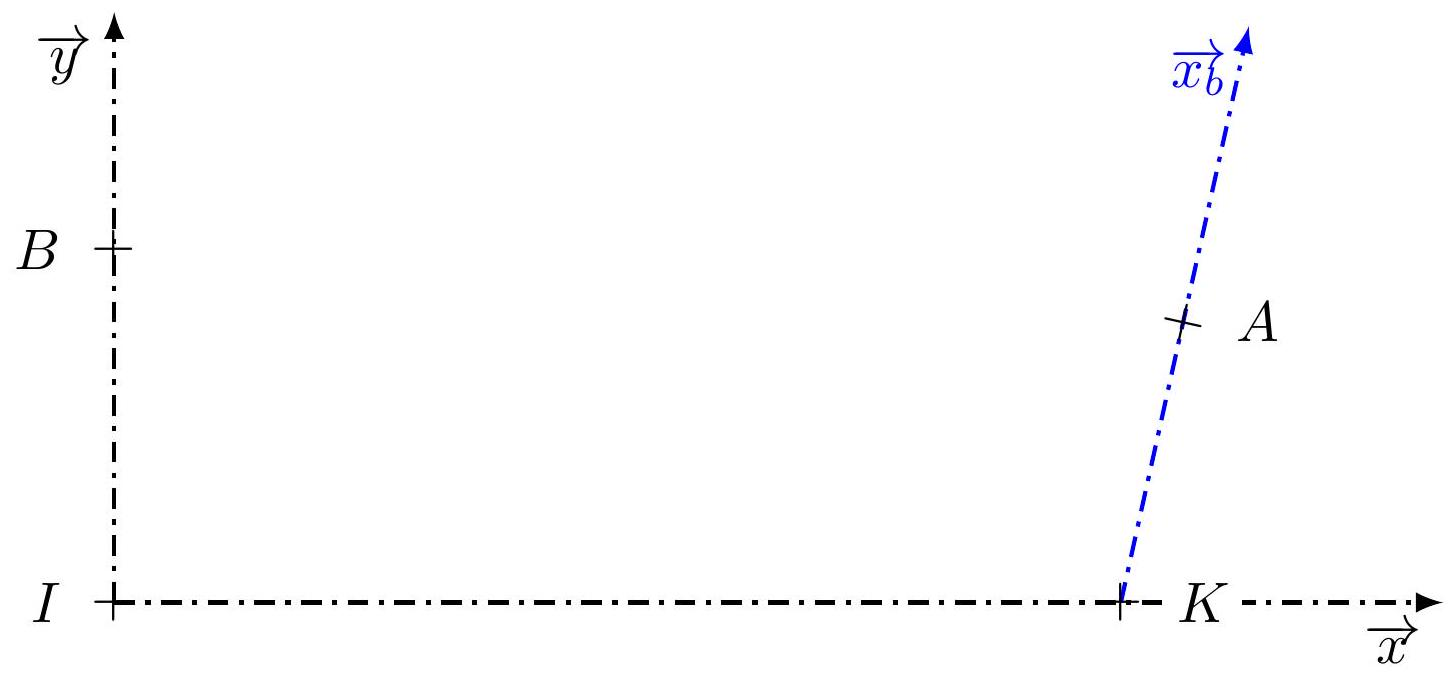
\includegraphics[width=.8\linewidth]{2024_12_06_8b2ce2e701dae8972925g-25(2)}

DR B : Figures de calcul - Question 4\\
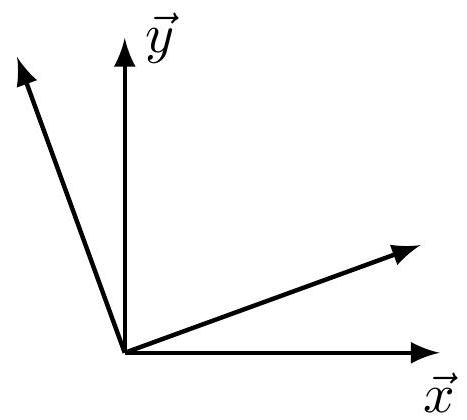
\includegraphics[width=.8\linewidth]{2024_12_06_8b2ce2e701dae8972925g-25(1)}\\
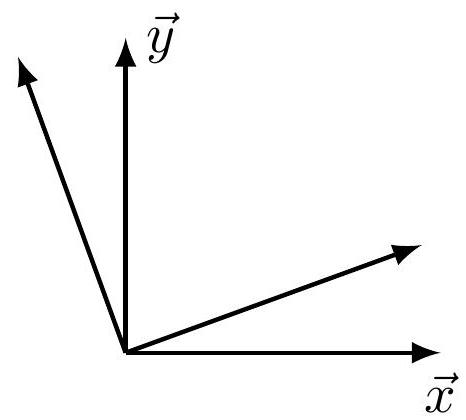
\includegraphics[width=.8\linewidth]{2024_12_06_8b2ce2e701dae8972925g-25}

DR C : Évolution de la tension Vcna - Question 41\\
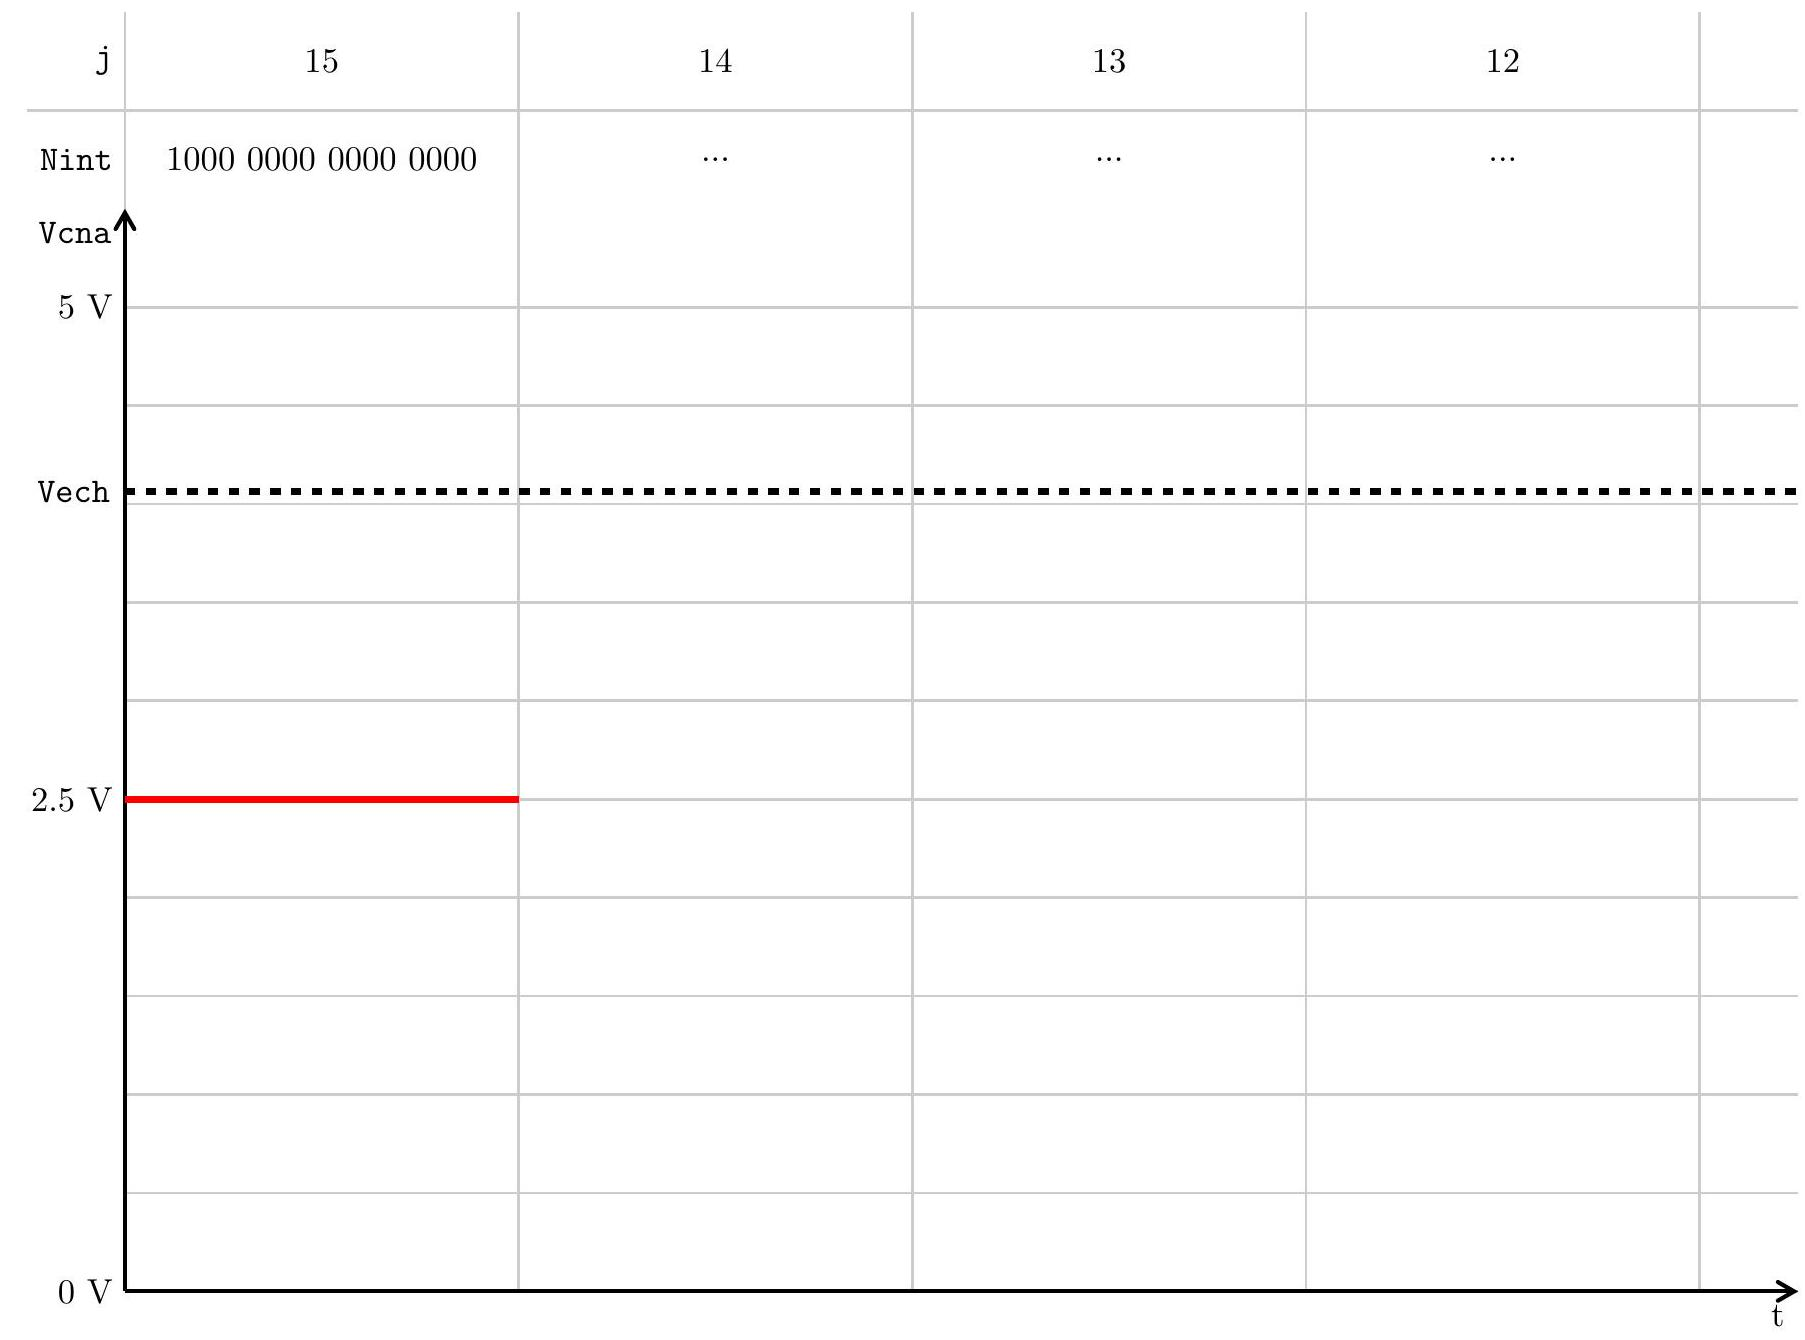
\includegraphics[width=.8\linewidth]{2024_12_06_8b2ce2e701dae8972925g-26(1)}

DR D : Mailles actives - Question 49\\
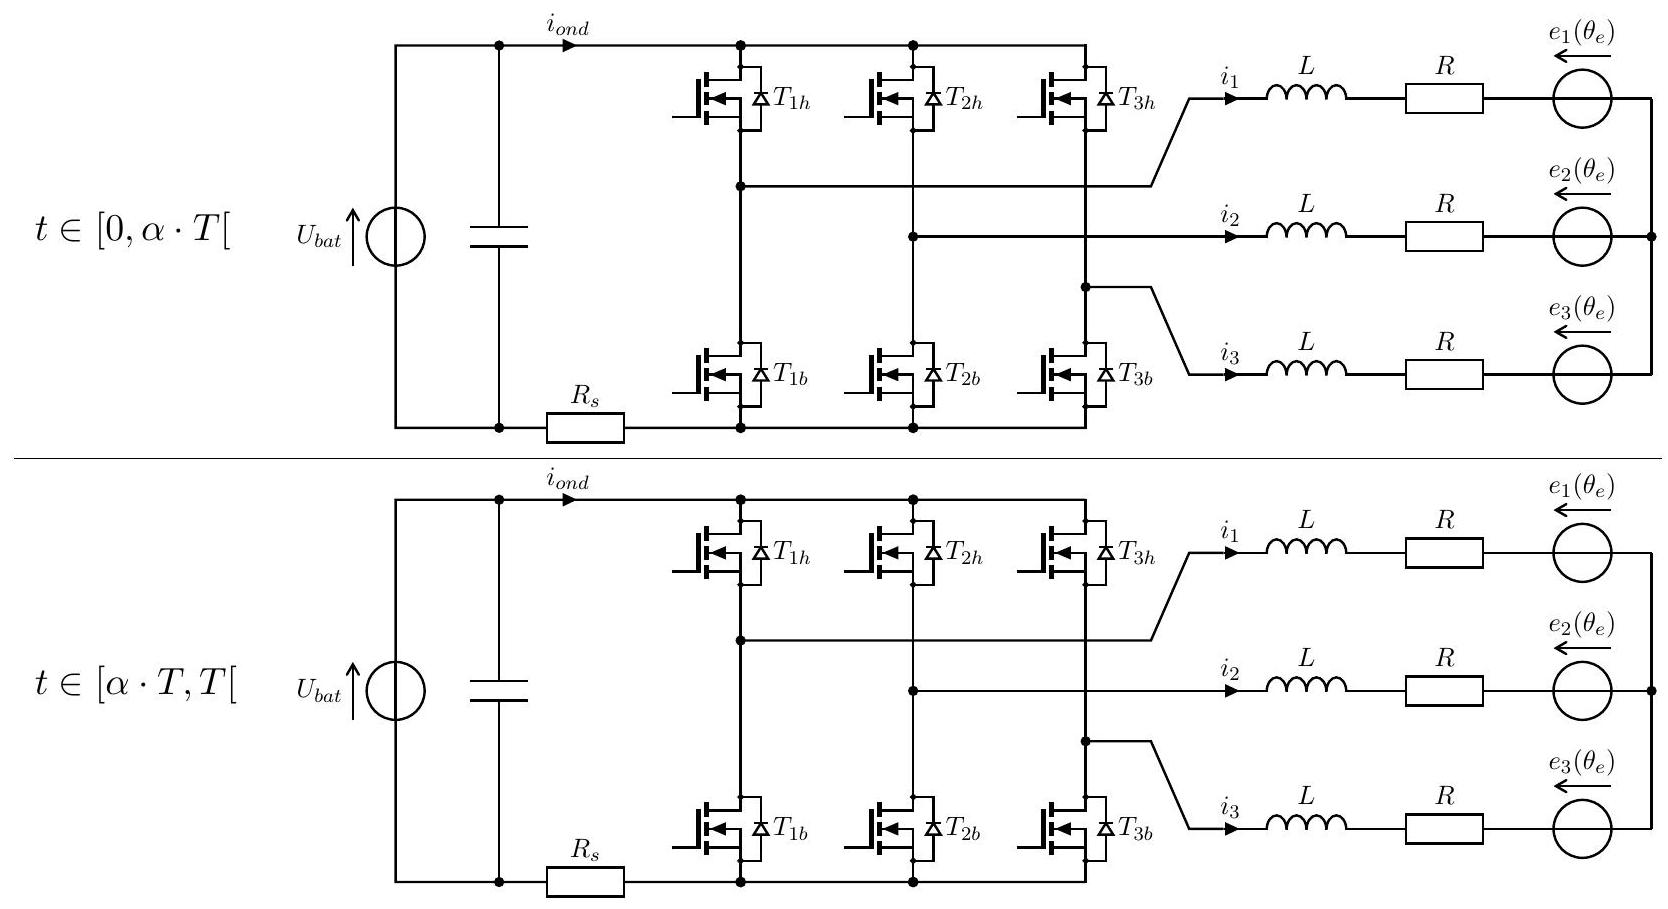
\includegraphics[width=.8\linewidth]{2024_12_06_8b2ce2e701dae8972925g-26}

\begin{enumerate}
  \item 
\end{enumerate}
%

